\documentclass[12pt, a4paper]{report}
\usepackage[italian]{babel}
\usepackage[T1]{fontenc}
\usepackage[utf8]{inputenc}
\usepackage{geometry}
\geometry{margin=2.5cm}
\usepackage{setspace}
\onehalfspacing
\usepackage{amsmath}
\usepackage{graphicx}
\graphicspath{{./images/}} % Specifica la cartella delle immagini
\usepackage{subcaption}    % Per sottofigure (alternativa più moderna: subcaption)
\usepackage{booktabs}      % Per tabelle più professionali
\usepackage{tabularx}     % Tabelle a larghezza fissa con colonne che vanno a capo
\usepackage{pgfplots}     % Grafici (curve di accumulo, confronti per profilo)
\pgfplotsset{compat=1.18}
\usepackage[authoryear,round,sort]{natbib}
\usepackage{url}
\usepackage{hyperref}
\usepackage{eurosym}
\usepackage{xcolor}
\hypersetup{colorlinks=true, linkcolor=black, citecolor=black, urlcolor=black,
  pdftitle={Adeguatezza pensionistica e autonomia previdenziale: riforme del sistema pensionistico italiano e strategie di integrazione complementare per i nuovi entranti nel mercato del lavoro},
  pdfauthor={Andrea Ferraboli},
  pdfsubject={Tesi di laurea triennale in Economia e Management, Universita degli Studi di Milano},
  pdfkeywords={previdenza, sistema pensionistico, NDC, adeguatezza, sostenibilita, previdenza complementare},
  pdflang={it-IT}}
% Consente la spezzatura delle URL lunghe in bibliografia (evita sbordi nel margine)
\Urlmuskip=0mu plus 1mu\relax
\def\UrlBreaks{\do\/\do\.\do\-\do\_\do\=\do\?\do\&\do\#\do\a\do\b\do\c\do\d\do\e\do\f\do\g\do\h\do\i\do\j\do\k\do\l\do\m\do\n\do\o\do\p\do\q\do\r\do\s\do\t\do\u\do\v\do\w\do\x\do\y\do\z\do\0\do\1\do\2\do\3\do\4\do\5\do\6\do\7\do\8\do\9}
\newcommand{\todo}[1]{\textcolor{red}{\textbf{[TODO: #1]}}}
% Stile economista: \cite default diventa parentetico (Autore, anno).
% Per le citazioni in cui l'autore e gia nominato nel testo si usa \citet
% (Autore (anno)) oppure \citeyearpar (solo l'anno tra parentesi).
\let\cite\citep

\title{%
    \textbf{Adeguatezza pensionistica e autonomia previdenziale:}\\[0.4em]
    \normalsize riforme del sistema pensionistico italiano e strategie di integrazione complementare per i nuovi entranti nel mercato del lavoro\\[0.5em]
}
\author{Andrea Ferraboli}

% Frontespizio: relatore, correlatore (opzionale), matricola, anno accademico
\makeatletter
\newcommand{\relatore}[1]{\def\@relatore{#1}}
\newcommand{\correlatore}[1]{\def\@correlatore{#1}}
\newcommand{\matricola}[1]{\def\@matricola{#1}}
\newcommand{\annoaccademico}[1]{\def\@anno{#1}}
\makeatother

\relatore{Michele Santoni}
\matricola{38241A} % sostituire con la propria matricola
\annoaccademico{2025/2026}

\begin{document}

\makeatletter
\begin{titlepage}%
    \thispagestyle{empty}%
    %\null\vskip1in%
    \begin{center}
        % Logo EMA (Economia & Management)
        
\includegraphics[width=0.22\textwidth]{Unimi-logo.png}

        \vspace{0.8cm}

        {\LARGE \textbf{Università degli Studi di Milano}} \\[0.4cm]
        {\large Facoltà di Scienze Politiche Economiche e Sociali} \\[0.2cm]
        {\normalsize Corso di Laurea Triennale in Economia e Management}

        \vspace{0.8cm}

        % Sigillo Università degli Studi di Milano
        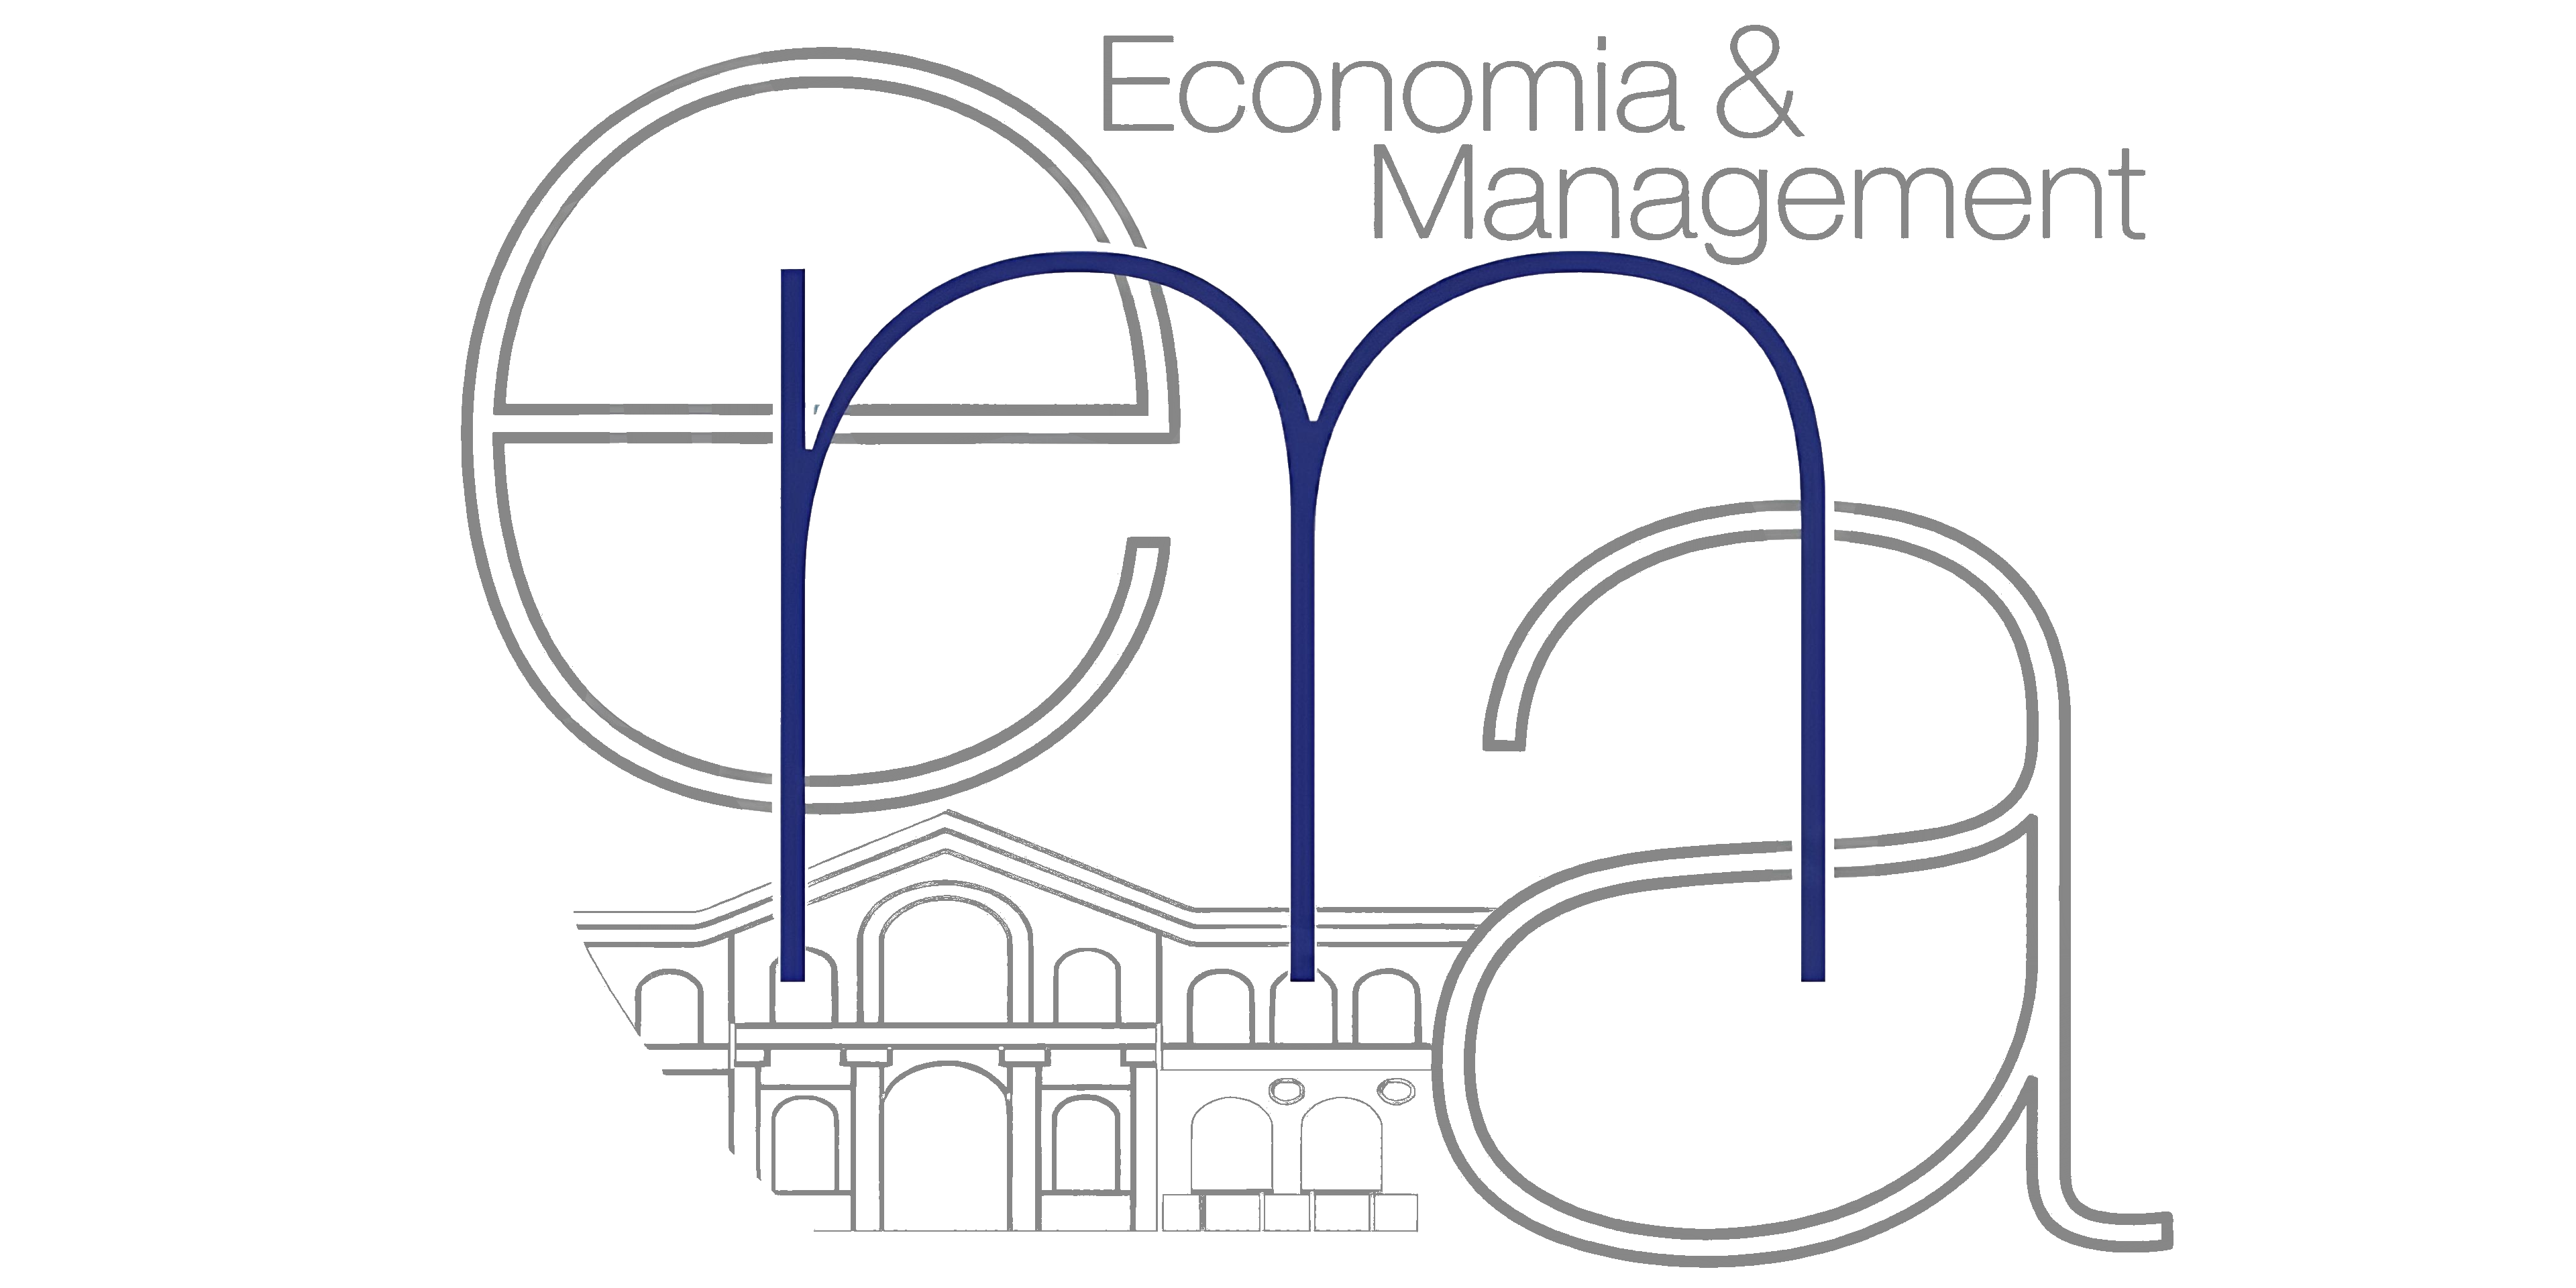
\includegraphics[width=0.35\textwidth]{logo_ema.png}
    \end{center}
    \begin{center}
% 		{\Large\uppercase\expandafter{\@title}}
    \begin{doublespace}
        {\large\uppercase\expandafter{\@title}}
    \end{doublespace}
    \end{center}
    \vfill
    \begin{description}
    \item[Relatore:] \@relatore
    \end{description}
    \vskip0.3in
    \null\hfill
    \parbox{1.5in}{
      Tesi di: \\
      \expandafter{\@author}
      \\ Matricola: \@matricola
      }
    \vfill
    \begin{center}
     \large   Anno Accademico \@anno
    \end{center}
    \newpage
  \end{titlepage}%
\makeatother

\tableofcontents

% !TeX root = ../second_main.tex
\chapter*{Introduzione}
\addcontentsline{toc}{chapter}{Introduzione}

% --- §0 EPIGRAFE -------------------------------------------------------
\begin{flushright}
\itshape
«Un sistema pensionistico non è una macchina\\
per pagare assegni: è un meccanismo\\
per redistribuire il rischio tra le generazioni.»\\[4pt]
\upshape
Elsa Fornero, \textit{Chi ha paura delle riforme} (2018)
\end{flushright}

\vspace{1em}

% --- §1 AGGANCIO NARRATIVO ---------------------------------------------
\noindent
Il dibattito previdenziale italiano ha storicamente privilegiato due domande:
\textit{quando} si può andare in pensione e \textit{quanto} costerà farlo.
Entrambe sono legittime. Entrambe, però, presuppongono come risolto il problema
più profondo: \textbf{se} il sistema è in grado di garantire a chi lavora oggi
un'esistenza dignitosa nella vecchiaia. È da questa terza domanda che muove la
presente tesi.

La previdenza pubblica obbligatoria risponde a fallimenti di mercato documentati
dalla teoria economica: i mercati privati non riescono a offrire copertura completa
contro il rischio demografico aggregato, le asimmetrie informative distorcono
l'offerta assicurativa, e la miopia intertemporale degli individui genera risparmi
sistematicamente insufficienti in assenza di un obbligo contributivo
\cite{Artoni2014, Bosi2018}. Nel sistema a ripartizione adottato dall'Italia,
i lavoratori attivi finanziano le pensioni degli anziani coevi, nella fiducia che
le generazioni successive faranno altrettanto: un patto intergenerazionale che
funge da meccanismo di redistribuzione del rischio demografico collettivo
\cite{Bosi2018}.

Un sistema alternativo, quello a capitalizzazione, lega il rendimento ai mercati
finanziari anziché alla crescita del PIL. Il passaggio da un sistema all'altro 
comporta però un costo di transizione di estrema complessità per l'Italia, 
data una spesa pensionistica attestata al 15,4\% del PIL nel 2024 \cite{MEF_RGS2025}: 
la generazione che affronta il passaggio si troverebbe infatti a dover finanziare 
simultaneamente le pensioni già in erogazione e il proprio accumulo futuro. 
Il dibattito tra i due modelli, pur fondamentale sul piano teorico, si scontra 
quindi con ostacoli attuativi di notevole portata nel breve e medio periodo \cite{Artoni2014}.

La domanda che rimane aperta, e che quasi nessuna riforma ha mai affrontato
con rigore, riguarda l'adeguatezza delle prestazioni future. Il dibattito
previdenziale ha attraversato decenni di interventi che hanno modificato
\textit{come} si calcola la pensione (riforma Dini, 1995), \textit{quando}
ci si può ritirare (riforma Fornero, 2011), e \textit{quanto tempo prima}
è possibile farlo cedendo a pressioni di breve periodo (Quota~100 nel 2019,
Quota~103 nel 2023). Ciascuno di questi interventi ha risposto a una domanda
contingente senza tornare al problema fondativo: garantire a tutti, e non
soltanto ai lavoratori già prossimi alla quiescenza, una vecchiaia
economicamente sostenibile.

% --- §2 IL PARADOSSO CENTRALE -----------------------------------------
\section*{Il paradosso della sostenibilità senza adeguatezza}

Il sistema previdenziale italiano si trova in una condizione di
\textbf{sostenibilità fragile}. Dal punto di vista macroeconomico, la traiettoria
appare rassicurante: la spesa per pensioni si attesta al 15,4\% del PIL nel 2024
\cite{MEF_RGS2025}, valore elevato nel confronto europeo ma destinato a ridursi
strutturalmente dopo il picco previsto intorno al 2042-2044, quando l'ultima
coorte del \emph{baby boom} raggiungerà l'età pensionabile portando il rapporto
spesa/PIL vicino al 17\%, per poi scendere al di sotto del 14\% nel 2070 grazie
all'applicazione generalizzata del metodo contributivo e alla stabilizzazione del
rapporto demografico tra pensionati e occupati \cite{MEF_RGS2025}.

Questa traiettoria discendente è il prodotto di una scelta tecnica con un costo
sociale profondo. Il sistema contributivo nozionale (NDC,
\emph{Notional Defined Contribution}), introdotto dalla riforma Dini e
generalizzato dalla riforma Fornero, calcola la pensione come funzione dell'intera
vita lavorativa e la comprime sistematicamente all'aumentare della speranza di
vita, attraverso la revisione periodica dei coefficienti di trasformazione.
In formula, la pensione annua lorda è:

\begin{equation}
P = \frac{MC_{NDC}}{e_L}
\qquad \text{con} \qquad
MC_{NDC} = \sum_{j=1}^{L} C_j \,(1+g)^{L-j}
\label{eq:ndc}
\end{equation}

\noindent dove $MC_{NDC}$ è il montante contributivo nozionale,
$C_j = c \cdot S_j$ i contributi versati nell'anno $j$
(con $c$ aliquota contributiva e $S_j$ retribuzione),
$g$ il tasso di capitalizzazione nozionale pari alla media mobile quinquennale
del PIL nominale, $e_L$ la speranza di vita all'età di pensionamento $L$
\cite{Bosi2018, MEF_RGS2025}.

\paragraph{Applicazione numerica.}
Si consideri un lavoratore dipendente con 35 anni di contributi, retribuzione
lorda costante di 30.000 euro e aliquota $c = 33\%$ (contributi annui: 9.900 euro),
con tasso nozionale $g = 1{,}5\%$, assunto a fini esemplificativi come ipotesi
prudenziale di crescita del PIL nominale \cite{ISTATCapitalizzazione2025, ISTATCapitalizzazione2024, ISTATCapitalizzazione2023}.
\[
\begin{aligned}
MC_{NDC}
  &= 9.900 \cdot \frac{(1{,}015)^{35} - 1}{0{,}015} \\
  &\approx 9.900 \times 45{,}6 \\
  &\approx 451.440 \text{ euro}
\end{aligned}
\]

Con il coefficiente di trasformazione a 67 anni fissato al 5,608\% per il
biennio 2025-2026 \cite{MEF_RGS2025}, la pensione lorda annua è:

\[
P_{\text{lordo}} = 0{,}05608 \times 451.440 = 25.320 \text{ euro annui}
\]

Il confronto al lordo è però parziale: il trattamento fiscale e contributivo
di lavoratori e pensionati diverge in modo significativo. Il lavoratore versa
contributi a proprio carico pari al 9,19\% della retribuzione lorda \cite{INPSAliquote2023}(circa
2.757 euro), che riducono l'imponibile IRPEF; la sua aliquota media effettiva
complessiva si colloca attorno al 27,7\% sul lordo. 

Per capire in che misura la pensione riesca a sostituire il precedente reddito lavorativo, dobbiamo calcolare la pensione netta e confrontarla con l'ultimo stipendio netto. Il pensionato non versa contributi e gode di un regime fiscale disciplinato dall'art. 13 del Testo Unico delle Imposte sui Redditi (TUIR) \cite{TUIR917_1986}. Per un reddito di 25.320 euro, che rientra nello scaglione tra 8.500 e 28.000 euro (comma 3, lett. b), a cui si aggiunge la maggiorazione per i redditi tra 25.000 e 29.000 euro (comma 3-bis), la detrazione spettante nel 2025 è:

\[
D_{\text{pens}} = 700 + \left[ 1.255 \times \frac{28.000 - 25.320}{19.500} \right] + 50 \approx 922 \text{ euro}
\]

L'IRPEF lorda (23\% $\times$ 25.320 = 5.824 euro) si riduce così a 4.902 euro;
con le addizionali regionali e comunali (media nazionale 1,5\%, circa 380 euro), l'imposta totale è di 5.282 euro. L'aliquota media effettiva si attesta quindi al 20,9\%, per una pensione netta di:

\[
P_{\text{netto}} = 25.320 \times (1 - 0{,}209) = 20.038 \text{ euro annui}
= 1.541 \text{ euro mensili}
\]

Lo stipendio netto vale circa 21.700 euro annui (1.668 euro mensili). Il
\textbf{tasso di sostituzione netto} è quindi:

\[
TS_{\text{netto}} = \frac{20.038}{21.700} = 92{,}3\%
\]

contro l'84\% lordo. Il differenziale si spiega con l'assenza, per il
pensionato, dei contributi IVS (acronimo di Invalidità, Vecchiaia e Superstiti) che sul lavoratore equivalgono a un prelievo
implicito di quasi 10 punti percentuali. Questa asimmetria è rilevante nella
valutazione dell'adeguatezza: i confronti condotti esclusivamente su basi lorde
sottostimano il reddito disponibile del pensionato rispetto all'ultimo anno
di lavoro.

La correzione non attenua il problema demografico; lo inquadra meglio. Se il
coefficiente di trasformazione scende al 5,2\% nel 2040 per effetto dell'aumento
della speranza di vita, la pensione lorda cala a:

\[
P_{\text{lordo},2040} = 0{,}052 \times 451.440 = 23.475 \text{ euro}
\]

Applicando nuovamente l'art. 13 del TUIR su questo nuovo imponibile (la detrazione sale a circa 991 euro, senza maggiorazione perché il reddito è sotto i 25.000 euro), l'aliquota media effettiva scende al 20,3\%. La pensione netta diventa circa 18.715 euro, pari a 1.440 euro mensili. Il tasso di sostituzione netto scende così all'86,2\%: una perdita di 6,1 punti percentuali rispetto allo scenario base, conseguenza di un solo parametro su cui il lavoratore non esercita alcuna leva: la longevità aggregata della propria coorte.

Su carriere con discontinuità contributiva, tipiche della Generazione Z, le
proiezioni della Ragioneria Generale dello Stato portano il tasso di sostituzione
lordo dei dipendenti privati al 58,4\% nel 2070, dal 73,6\% del 2010
\cite{MEF_RGS2025}. Convertendo al netto, il guadagno fiscale è simmetrico tra
generazioni e non compensa la perdita strutturale di rendimento del sistema a
contribuzione definita. Un lavoratore entrato nel 1982 e pensionatosi nel 2020 ha
percepito un tasso di sostituzione lordo dell'81,5\%, pari a circa l'87\% al netto.
Un giovane entrato nel 2022 che andrà in pensione nel 2060 otterrà il 64,8\% lordo:
circa 17 punti percentuali in meno \cite{Censis_Confcooperative2026}. La previdenza
complementare risale al 66\% lordo \cite{MEF_RGS2025}, ma sull'ipotesi di adesione
piena che per i lavoratori discontinui rimane un'assunzione difficilmente
verificabile nella pratica.

La contraddizione è strutturale. \textbf{La sostenibilità finanziaria del sistema
è stata acquistata al prezzo dell'adeguatezza futura delle prestazioni.} Le riforme
hanno risolto il problema del come finanziare le pensioni di domani senza rispondere
al problema del se quelle pensioni saranno sufficienti a garantire una vecchiaia
dignitosa. Questo trade-off è il nucleo analitico attorno al quale si sviluppa
la presente tesi.

% --- §3 LE DOMANDE DI RICERCA -----------------------------------------
\section*{Le domande di ricerca}

La tesi si articola attorno a tre domande di ricerca strettamente interconnesse,
che procedono dal livello macroeconomico-istituzionale a quello individuale.

\begin{description}
\item[\textbf{Domanda 1 (adeguatezza).}]
Il sistema NDC italiano, nella sua configurazione attuale e nelle sue proiezioni di
lungo periodo, è in grado di garantire alle generazioni future un tenore di vita
dignitoso nella vecchiaia? In che misura il tasso di sostituzione atteso è compatibile
con le funzioni previdenziale, assicurativa e assistenziale che la teoria economica
assegna alla previdenza pubblica \cite{Bosi2018}?

\item[\textbf{Domanda 2 (riforme strutturali).}]
Quali interventi di politica economica, dai correttivi tecnici al sistema NDC
(revisione delle aliquote di capitalizzazione, garanzie di minimo pensionistico,
flessibilità attuarialmente neutra dell'età di uscita) al più radicale
\emph{Contributo sull'Automazione} come fonte alternativa di finanziamento,
possono correggere il trade-off tra sostenibilità e adeguatezza?

\item[\textbf{Domanda 3 (agentività individuale).}]
In quale misura il singolo lavoratore, in un sistema che ha progressivamente
trasferito su di lui il rischio demografico e il rischio di longevità, mantiene
la capacità di agire sulla propria condizione futura? E questa agentività è
equamente distribuita tra chi ha carriere regolari e chi le ha discontinue, o
costituisce essa stessa un ulteriore fattore di disuguaglianza?
\end{description}

% --- §4 STRUTTURA DELLA TESI ------------------------------------------
\section*{Struttura della tesi}

La tesi è organizzata in tre parti logicamente consequenziali, che corrispondono a
tre livelli di analisi progressivamente più orientati all'azione.

La \textbf{Prima Parte} costruisce le fondamenta teoriche, istituzionali e storiche
del sistema previdenziale italiano. Il primo capitolo ricostruisce la logica economica
della previdenza pubblica (fallimenti del mercato, funzione del patto
intergenerazionale, modelli a ripartizione e a capitalizzazione) per poi
descrivere il funzionamento del sistema NDC e calcolarne il tasso di rendimento
implicito, con riferimento alla letteratura canonica \cite{Bosi2018, Artoni2014}.
Una sezione di sintesi storica chiude il capitolo ripercorrendo l'evoluzione del
sistema pensionistico italiano dalla riforma Amato del 1992 alla riforma Fornero
del 2011, analizzando le deroghe di Quota 100, Quota 102 e Quota 103 come
manifestazioni di un conflitto irrisolto tra equità attuariale e consenso elettorale.

La \textbf{Seconda Parte} affronta il nucleo del problema, analizzando il trade-off
tra sostenibilità e adeguatezza. Il secondo capitolo funge da \textbf{diagnosi
empirica}: attraverso le proiezioni di lungo periodo della Ragioneria Generale dello
Stato \cite{MEF_RGS2025}, identifica il picco di spesa atteso e quantifica il
deterioramento del tasso di sostituzione per le generazioni future, confrontando
scenari con e senza previdenza complementare. Il terzo capitolo passa dalla diagnosi
alle \textbf{soluzioni}, mappando le proposte di riforma strutturale in discussione
nel dibattito internazionale, dalla letteratura di \textsc{VoxEU} ai contributi di
\textsc{Lavoce.info} e del \textsc{CERP}, valutandone l'efficacia e la fattibilità
politica.

La \textbf{Terza Parte} sposta il fuoco dall'analisi macroeconomica di sistema
all'azione del singolo, ponendo una domanda precisa: in un contesto di riforme
rinviate e rischio demografico crescente, quanto può davvero fare il lavoratore
per tutelarsi? Il quarto capitolo, attraverso simulazioni su diversi profili di
carriera della Generazione Z, esamina la \textbf{regressività implicita} della
previdenza complementare e delinea un \textit{framework} di pianificazione
individuale basato su risparmio e riscatti contributivi, condizionato però da
soglie minime di reddito.

Le \textbf{Conclusioni} raccolgono le risposte alle tre domande di ricerca e
formulano raccomandazioni di policy, distinguendo tra misure adottabili nel breve
periodo, senza necessità di riforma organica, e interventi strutturali di lungo
respiro.
\chapter{Le Fondamenta del Sistema Previdenziale: Teoria e Scelte Storiche}

Un sistema pensionistico non è mai neutro. Dietro ogni aliquota contributiva, ogni formula di calcolo, ogni soglia anagrafica, c'è una scelta su chi paga e chi riceve, su quale generazione sostiene il peso e quale lo scarica nel tempo. Per capire la crisi strutturale del sistema italiano occorre partire dalle fondamenta: le ragioni teoriche che giustificano l'intervento dello Stato, la logica matematica dei modelli di finanziamento, e le scelte storiche che hanno plasmato un'architettura previdenziale ancora gravata dalle sue contraddizioni originarie.

\section{Le ragioni dell'intervento pubblico}

\subsection{Funzione previdenziale, assicurativa e assistenziale}

Il sistema pensionistico pubblico svolge tre funzioni distinte che nella realtà si sovrappongono, ma che la teoria tiene accuratamente separate. La prima è la funzione previdenziale: garantire ai lavoratori in pensione un tenore di vita simile a quello raggiunto durante l'attività, a condizione che abbiano contribuito in misura adeguata. La seconda è la funzione assicurativa: proteggere i cittadini dal rischio di riduzione del reddito legato a eventi come l'invalidità, la morte prematura del capofamiglia, o semplicemente una longevità superiore alle aspettative. La terza è la funzione assistenziale: garantire un reddito minimo a chi non ha contribuito abbastanza per vivere in modo dignitoso, indipendentemente dalla storia lavorativa~\cite{Bosi2018, RosenGayerRapallini2023}.

Le tipologie di pensione corrispondono a queste funzioni in modo preciso~\cite{RosenGayerRapallini2023}:

\begin{center}
\begin{tabularx}{\textwidth}{|l|>{\raggedright\arraybackslash}X|>{\raggedright\arraybackslash}X|}
\hline
Tipologia & Beneficiario & Funzione prevalente \\
\hline
Vecchiaia & Ritirato per limiti di età & Previdenziale / assicurativa \\
\hline
Anzianità (anticipata) & Ritirato per anni di contribuzione & Previdenziale / assicurativa \\
\hline
Ai superstiti & Familiare del lavoratore deceduto & Assistenziale / previdenziale \\
\hline
Invalidità & Inabile al lavoro & Assicurativa / assistenziale \\
\hline
Sociale & Sprovvisto di reddito e incapace di lavorare & Assistenziale \\
\hline
\end{tabularx}
\end{center}

La distinzione rileva sul piano dell'analisi positiva perché ciascuno strumento ha una propria logica di finanziamento e di accesso. La pensione di invalidità risponde a un criterio medico, mentre quella di anzianità risponde a un criterio contributivo legato agli anni di versamenti accumulati dal lavoratore. Confondere i due piani produce distorsioni che si materializzano nei bilanci dell'ente previdenziale anni o decenni più tardi.

In Italia, tra gli anni Settanta e Ottanta, questi strumenti furono spesso impiegati al di fuori della loro logica originaria. Le pensioni di invalidità, in alcune aree del Mezzogiorno, vennero talvolta utilizzate come forma di sostegno al reddito in assenza di un vero reddito minimo garantito. Le pensioni di anzianità, rese accessibili da requisiti relativamente bassi introdotti con la riforma del 1969, divennero invece uno dei principali canali di prepensionamento industriale: nelle grandi imprese del Nord, le ristrutturazioni e le chiusure di reparti potevano essere accompagnate dall’uscita anticipata dei lavoratori, con una parte rilevante dei costi trasferita al sistema previdenziale~\cite{Bosi2018, Ferrera_1996}.

Ogni lavoratore mandato in pensione a cinquant'anni invece che a sessantacinque rappresentava quindici anni di prestazione aggiuntiva rispetto a quanto tecnicamente dovuto, senza una corrispondente copertura contributiva. Questo accumulo è quello che Bosi chiama ``debito previdenziale'': la differenza tra il valore attuale di tutte le pensioni promesse e il valore attuale di tutti i contributi futuri attesi. Una volta formatosi, è quasi impossibile ridurlo senza toccare i diritti acquisiti di chi già percepisce la pensione, oppure scaricando il costo sui lavoratori attivi attraverso aliquote più alte~\cite{Bosi2018}.

\subsection{Fallimenti del mercato e miopia individuale}

In presenza di mercati completi e di agenti pienamente razionali, l'intervento pubblico in materia previdenziale sarebbe difficile da giustificare sul piano dell'efficienza: per il primo teorema dell'economia del benessere, l'allocazione di mercato risulterebbe già Pareto-efficiente. L'individuo dell'ipotesi del ciclo vitale di Modigliani accumulerebbe risparmio durante la vita attiva per smobilizzarlo in vecchiaia, livellando il consumo nel tempo. La realtà si discosta da queste ipotesi su più fronti, e l'intervento pubblico risponde a fallimenti documentati~\cite{Bosi2018}.

I mercati assicurativi privati non riescono a offrire copertura completa contro il rischio di inflazione e contro i rischi sistemici, che per definizione non si diversificano, mentre la moltiplicazione di fondi privati in concorrenza genera costi di gestione e marketing che erodono il rendimento netto del pensionato~\cite{RosenGayerRapallini2023}. Vi è poi la miopia individuale, per cui gli esseri umani sistematicamente sottovalutano il futuro lontano e sovrastimano la propria capacità di risparmio volontario, al punto che senza un obbligo contributivo molti lavoratori arriverebbero alla vecchiaia senza riserve sufficienti~\cite{RosenGayerRapallini2023}.

L'azzardo morale completa il quadro. Un lavoratore che non risparmia sa che lo Stato non lo lascerà in miseria nella vecchiaia; questa convinzione genera un incentivo perverso che l'obbligatorietà del contributo risolve ex ante. A questo si aggiunge la selezione avversa: se la contribuzione fosse volontaria, i lavoratori più giovani e produttivi uscirebbero dal sistema lasciando solo i soggetti a maggior rischio, la base contributiva si restringerebbe e il sistema imploderebbe~\cite{RosenGayerRapallini2023}.

\section{I modelli di finanziamento a confronto}

\subsection{Il sistema a Ripartizione (PAYG): il patto intergenerazionale}

In un sistema a ripartizione i contributi versati oggi all'INPS escono immediatamente dall'ente per pagare le pensioni di chi è già in quiescenza. Il lavoratore di oggi finanzia il pensionato di oggi; quando raggiungerà a sua volta l'età pensionabile, sarà la generazione successiva a coprire il suo assegno. Il sistema regge finché ogni generazione accetta implicitamente questo accordo e finché le condizioni demografiche ed economiche non cambiano in modo tale da rendere impossibile l'adempimento~\cite{Bosi2018}.

Bosi definisce il meccanismo ``patto intergenerazionale'', perché il rendimento non dipende dai mercati finanziari ma dalla dimensione e dalla produttività della generazione successiva: una forza lavoro futura numerosa e produttiva sostiene pensioni adeguate, mentre una forza lavoro scarsa e a bassa crescita salariale comprime il monte contributivo disponibile~\cite{Bosi2018}.

Per formalizzare il meccanismo si usa il modello a generazioni sovrapposte, nella formulazione che da Samuelson e Diamond in poi costituisce il riferimento canonico per l'analisi dei sistemi a ripartizione~\cite{Samuelson1958, Diamond1965, Bosi2018}. Siano \(N_t\) gli anziani (pensionati) e \(N_{t+1}\) i giovani (lavoratori). La popolazione cresce al tasso costante \(n\), per cui \(N_{t+1} = (1+n)N_t\). Il parametro \(n\) misura il tasso di crescita della forza lavoro da un periodo al successivo: un valore \(n = 0{,}01\) indica che la nuova generazione di lavoratori è l'1\% più numerosa della precedente. Nelle economie mature contemporanee, con tassi di fertilità sotto il livello di rimpiazzo, \(n\) è prossimo a zero o negativo~\cite{Bosi2018, RosenGayerRapallini2023}.

Il salario per lavoratore è \(S_t\) e cresce al tasso di produttività \(m\). L'aliquota contributiva è \(c\). La pensione pro capite in ripartizione è~\cite{Bosi2018, RosenGayerRapallini2023}:

\[
P_{t+1}^{\text{ripartizione}} = c \cdot S_{t+1} \cdot \frac{N_{t+1}}{N_t} = c \cdot S_t (1+m)(1+n)
\]

Il tasso di rendimento implicito del sistema è pari a \(m+n\), ossia la somma del tasso di crescita della produttività e del tasso di crescita della popolazione occupata. In ripartizione, il rendimento non dipende dai mercati finanziari ma dall'andamento dell'economia reale~\cite{RosenGayerRapallini2023}.

Con \(c=0{,}33\), \(S=30.000\) euro, \(m=0{,}02\), \(n=0{,}01\) e un rapporto di 2 lavoratori per ogni pensionato, la pensione annua pro capite è:

\[
P = 0{,}33 \times 30.000 \times 1{,}02 \times 1{,}01 \times 2 = 20.430 \text{ euro}
\]

Se la demografia peggiora e \(n\) scende a \(-0{,}01\), il monte contributivo si contrae e ogni pensionato riceve di meno. Il sistema è strutturalmente esposto alla demografia: un calo della natalità, un allungamento della speranza di vita, una contrazione dell'occupazione riducono il monte contributivo o allungano il periodo di erogazione~\cite{RosenGayerRapallini2023}.

\subsection{Il sistema a Capitalizzazione (Fully Funded): rischi e opportunità}

Nel sistema a capitalizzazione ogni lavoratore accumula su un conto individuale i propri contributi, investiti sui mercati finanziari. Al pensionamento, la pensione equivale al montante accumulato rivalutato al tasso di rendimento \(r\), senza alcuna redistribuzione tra generazioni~\cite{Bosi2018, RosenGayerRapallini2023}:

\[
P_{t+1}^{\text{capitalizzazione}} = c \cdot S_t (1+r)
\]

Il confronto tra i due sistemi si riduce al confronto tra \(r\) e \((m+n)\). Il teorema di Samuelson-Aaron formalizza questa condizione~\cite{Samuelson1958, Aaron1966}: il PAYG è efficiente solo quando il tasso di crescita demografica ed economica supera stabilmente il rendimento reale del capitale. Nelle economie mature, con popolazioni stagnanti e rendimenti reali di lungo periodo sui mercati finanziari intorno al 4-5\%, la capitalizzazione sembrerebbe avvantaggiata. I rischi strutturali ne limitano però la superiorità~\cite{Bosi2018}.

Il rischio di mercato è il più evidente: crisi finanziarie come quella del 2008 possono azzerare decenni di accumulo senza meccanismi compensativi collettivi. Il rischio di longevità si aggiunge perché vivere più a lungo del previsto esaurisce il montante, e le rendite vitalizie offerte dal mercato sono costose proprio perché la longevità è un rischio aggregato non diversificabile~\cite{RosenGayerRapallini2023}.

Il rischio di inflazione merita un'analisi più articolata. L'effetto Fisher descrive il comportamento dei tassi nominali sui nuovi strumenti emessi dopo un aumento dell'inflazione. Il punto critico è che un fondo pensione è fatto in larga parte di titoli acquistati anni o decenni prima, quando l'inflazione era bassa e i tassi nominali erano corrispondentemente contenuti. Quelle posizioni sono aperte, i loro rendimenti sono fissi per contratto e non possono essere rivalutate retroattivamente: un portafoglio obbligazionario che rende il 3-4\% nominale subisce un'erosione reale significativa se l'inflazione sale al 7\% nei cinque anni precedenti il pensionamento. A questo si aggiunge un profilo istituzionale: nei mercati europei del dopoguerra, e in Italia durante la stagflazione degli anni Settanta, i tassi d'interesse erano soggetti a controlli politici che impedivano al meccanismo correttivo di attivarsi~\cite{RosenGayerRapallini2023}. I titoli indicizzati all'inflazione, come i BTP Italia o i CCT a cedola variabile, attenuano questo rischio per la quota di portafoglio che vi è investita, ma restano una componente minoritaria dei patrimoni previdenziali e non proteggono i titoli a cedola fissa già in portafoglio, sui quali la perdita reale resta integrale.

In ripartizione le pensioni sono spesso indicizzate all'inflazione per legge, e se i salari nominali crescono con l'inflazione crescono anche i contributi versati. Il rischio diventa collettivo e lo Stato agisce come garante residuale. Questo meccanismo cede tuttavia in caso di stagflazione: i contributi ristagnano perché i salari reali sono fermi, ma le pensioni indicizzate continuano a salire in termini nominali, producendo un disavanzo strutturale. L'effetto Fisher opera sui flussi futuri e non sugli stock passati, funziona imperfettamente nei mercati regolamentati, e non risolve il problema dell'incertezza individuale di lungo periodo~\cite{RosenGayerRapallini2023}.

\section{La genesi e l'evoluzione del sistema italiano}

\subsection{Dalle origini al dopoguerra: il passaggio alla ripartizione}

Il sistema pensionistico italiano nasce come sistema a capitalizzazione. Le prime pensioni di invalidità e vecchiaia furono istituite nel 1864 per i soli dipendenti statali; nel 1919, con il decreto legislativo 603, l'assicurazione obbligatoria fu estesa ai lavoratori dipendenti privati dell'industria, dell'agricoltura e dei servizi, gestita dalla Cassa Nazionale delle Assicurazioni Sociali~\cite{CERP2008}.

Due guerre mondiali e l'inflazione bellica e post-bellica distrussero le riserve accumulate. Con la legge 218 del 1952 si introduce il trattamento minimo di pensione e il sistema entra in una fase mista in cui il contributo pubblico diretto affianca i contributi dei lavoratori, operando già parzialmente con logica di ripartizione~\cite{CERP2008, Bosi2018}. Il passaggio definitivo avviene nel 1969, con la riforma Brodolini (legge 153/1969). La scelta non fu dettata soltanto da ragioni tecniche: i sindacati chiedevano pensioni più alte nell'immediato, e con la ripartizione bastava trasferire subito una quota più alta dei salari correnti, scaricando il costo sui lavoratori attivi anziché su riserve pregresse~\cite{Fondapol}.

L'Italia del 1969 aveva una struttura demografica favorevole. Come scrive Favero su Lavoce.info, nessuno fece i conti su cosa sarebbe successo quando quel rapporto si fosse invertito. La scelta di alzare subito le prestazioni correnti senza costituire coperture pluriennali aprì un disavanzo previdenziale crescente, nascosto dall'inflazione per un decennio e poi diventato visibile quando la crescita rallentò~\cite{LavoceRiformaDini}.

\subsection{Il metodo retributivo: logica, distorsioni e debito implicito}

L'abbandono della capitalizzazione coincise con l'adozione del metodo retributivo per il calcolo della pensione. La pensione non dipende dai contributi effettivamente versati, ma dalla retribuzione percepita negli ultimi anni di lavoro moltiplicata per un tasso legato agli anni di contribuzione~\cite{Bosi2018}:

\[
P = \tau \times W_{\text{pensionabile}}
\]

dove \(\tau\) è il tasso di rendimento (2\% per anno di contribuzione, da un minimo del 40\% per 20 anni a un massimo dell'80\% per 40 anni) e \(W_{\text{pensionabile}}\) è la retribuzione di riferimento rivalutata per inflazione più 1\%~\cite{RosenGayerRapallini2023}.

Il metodo retributivo scollega quasi completamente i benefici dai contributi versati, perché un lavoratore che ha guadagnato poco per trent'anni e molto negli ultimi cinque riceve una pensione ben superiore a quanto giustificato dai suoi versamenti complessivi, con un rendimento implicito sui contributi sistematicamente superiore al tasso di crescita dell'economia, in violazione del principio di sostenibilità finanziaria~\cite{LavoceRiformaDini}. Le prime avvisaglie di squilibrio emergono negli anni Ottanta: il rallentamento della crescita, il calo demografico e la riduzione del tasso di occupazione comprimono il monte contributivo, mentre le promesse retributive continuano a pesare sul bilancio INPS a ritmo crescente. Il debito previdenziale non compariva nei bilanci ufficiali, ma era reale come il debito esplicito, e la crisi degli anni Novanta avrebbe reso quel debito improvvisamente visibile~\cite{LavoceRiformaDini, Bosi2018}.

\subsection{La stagione delle riforme: dal metodo retributivo al sistema NDC}

La riforma Amato del 1992 (decreto legislativo 503/1992) è il primo intervento organico: aumenta l'età pensionabile, porta il requisito contributivo minimo per la pensione di vecchiaia da 15 a 20 anni, e amplia la finestra temporale di riferimento per il calcolo della retribuzione pensionabile. Si tratta di un intervento sul perimetro del sistema, senza toccare la logica di fondo del metodo retributivo~\cite{Bosi2018}.

La riforma strutturale arriva con il governo Dini nel 1995 (legge 335/1995), in un contesto di pressione per l'ingresso nell'euro con il debito pubblico già oltre il 120\% del PIL. L'obiettivo è sostituire il sistema retributivo con il sistema contributivo nozionale (NDC, Notional Defined Contribution): la pensione dipende dai contributi effettivamente versati durante l'intera vita lavorativa, capitalizzati a un tasso agganciato alla crescita del PIL. La scelta di usare la crescita del PIL come tasso di capitalizzazione ha una coerenza interna precisa: in un sistema a ripartizione, come dimostrato nel modello a generazioni sovrapposte, il tasso di rendimento implicito è proprio \((1+m)(1+n)\), ossia la crescita dell'economia. Usare quel tasso come coefficiente di accumulazione virtuale rendeva il sistema internamente coerente e, almeno in teoria, attuarialmente neutrale, nel senso che a parità di contributi versati il valore atteso della pensione è lo stesso per tutti e il sistema non trasferisce risorse né tra individui né tra generazioni oltre la crescita dell'economia~\cite{RosenGayerRapallini2023}.

La formula della pensione annuale lorda nel sistema NDC è:

\[
P = \alpha_L \cdot M_C^{NDC}
\]

dove \(\alpha_L\) è il coefficiente di trasformazione che dipende dalla speranza di vita residua all'età di pensionamento \(e_L\), e \(M_C^{NDC}\) è il montante contributivo, ottenuto come somma capitalizzata di tutti i contributi versati:

\[
M_C^{NDC} = \sum_{j=1}^{L} C_j \cdot (1+g)^{L-j}
\]

con \(g\) pari alla media mobile quinquennale del tasso di crescita del PIL nominale, \(C_j = c \cdot S_j\) e l'aliquota \(c = 0{,}33\) per i lavoratori dipendenti. Il coefficiente di trasformazione si ricava imponendo l'equilibrio finanziario tra montante e pensioni attese~\cite{RosenGayerRapallini2023}:

\[
M_C^{NDC} = \sum_{k=1}^{e_L} \frac{P}{(1+r_z)^{k-1}}
\quad \Longrightarrow \quad
P = \frac{M_C^{NDC}}{e_L}
\quad (\text{con } r_z = 0)
\]

Quanto più lunga è la speranza di vita al momento del pensionamento, tanto più piccolo è \(\alpha_L = 1/e_L\), e tanto più bassa è la pensione annua a parità di montante. Per il biennio 2023-2024 i coefficienti vigenti variano da un minimo del 4,270\% a 57 anni a un massimo del 6,655\% a 71 anni~\cite{RosenGayerRapallini2023}, e la revisione biennale li riduce ulteriormente al crescere della speranza di vita. È il meccanismo di aggiustamento automatico introdotto dalla riforma Dini e poi esteso dalla riforma Fornero ai requisiti di accesso~\cite{Bosi2018}; un'applicazione numerica completa del metodo, dal montante alla pensione netta, è già stata svolta nell'introduzione.

La riforma Dini applicava il sistema NDC integralmente solo a chi entrava nel mercato del lavoro dal 1 gennaio 1996. Chi aveva già 18 anni di contributi al 31 dicembre 1995 rimaneva interamente sotto il regime retributivo, anche per la parte maturata in seguito. Il risparmio effettivo sulla spesa pensionistica si sarebbe quindi materializzato solo decenni dopo, caricando sulle generazioni più giovani l'intero onere del riequilibrio e lasciando intatto il privilegio di chi era già profondamente radicato nel sistema~\cite{LavoceRiformaDini, Bosi2018}.

La risposta a questo gradualismo irrisolto arriva nel novembre 2011 con il decreto ``Salva Italia'' (decreto-legge 201/2011, convertito con legge 214/2011) del governo Monti, con lo spread a 570 punti base. La riforma Fornero estende il metodo contributivo a tutti i lavoratori a partire dal 1 gennaio 2012, unifica l'età pensionabile di vecchiaia a 67 anni per uomini e donne a partire dal 2019, e introduce il collegamento automatico dei requisiti di accesso alla speranza di vita: ogni due anni l'età richiesta per la pensione viene rivista in funzione delle variazioni della speranza di vita calcolate dall'Istat, così che a un allungamento della vita attesa corrisponda un posticipo dell'uscita dal lavoro. I risparmi stimati ammontavano a oltre 22 miliardi di euro entro il 2020~\cite{RepubblicaFornero2012}. La riforma si inserisce nel più ampio ciclo di interventi avviato nel 2004, al quale la Ragioneria Generale dello Stato attribuisce una riduzione del rapporto spesa/PIL di oltre 60 punti percentuali cumulati al 2060; alla sola riforma Fornero è ascrivibile circa un terzo di questo effetto~\cite{MEF_RGS2025_NdA, BosiGuerra2022}.

La risposta politica alla riforma si è tradotta in una serie di deroghe che hanno progressivamente eroso la coerenza attuariale del sistema. Quota 100 (decreto-legge 4/2019, triennio 2019-2021) consentiva il pensionamento con 62 anni di età e 38 di contributi. Quota 102, attiva per il solo 2022, aumentava i requisiti a 64 anni di età e 38 di contributi. Quota 103, introdotta per il 2023 e prorogata al 2024, ha fissato i requisiti a 62 anni di età e 41 di contribuzione, con la pensione calcolata integralmente con il metodo contributivo. Ciascuna di queste misure consente di percepire la pensione per più anni del previsto senza un corrispondente aumento del montante, scaricando il differenziale di costo sulla collettività e riproducendo, in forma attenuata, il meccanismo che la riforma Dini aveva cercato di interrompere~\cite{LavoceRiformaDini, MEF_RGS2025}.
\chapter{Il Corto Circuito: Analisi delle Criticità del Sistema Vigente}

\section*{2.0 Dal modello teorico alla dinamica delle riforme}

Le criticità emerse nel capitolo precedente non rimangono confinate alla dimensione astratta della teoria previdenziale, ma trovano una traduzione immediata nella storia istituzionale italiana. La logica del sistema a ripartizione chiarisce infatti che, quando il tasso di crescita della popolazione attiva rallenta e la produttività non è sufficiente a compensarne gli effetti, la sostenibilità del sistema dipende in misura crescente da due variabili decisive: l'età effettiva di uscita dal lavoro e l'adeguatezza del montante contributivo accumulato~\cite{Bosi2018, RosenGayerRapallini2023}. In altri termini, la tenuta finanziaria non è un fatto puramente contabile, ma il risultato di un equilibrio tra demografia, mercato del lavoro e regole di accesso alle prestazioni.

È precisamente in questo punto di intersezione che si collocano le riforme pensionistiche italiane degli ultimi decenni. Esse non vanno lette come una sequenza discontinua di correzioni tecniche, bensì come il tentativo di ricomporre una frattura aperta tra il principio attuariale introdotto con il sistema contributivo nozionale e la pressione politico-sociale verso canali di uscita anticipata dal mercato del lavoro~\cite{LavoceRiformaDini, MEFRGS2025}. La questione delle deroghe, delle quote e delle finestre di flessibilità non costituisce dunque un capitolo accessorio, ma il luogo in cui si manifesta con maggiore evidenza la tensione tra sostenibilità finanziaria, adeguatezza delle prestazioni e consenso distributivo.

Per questo motivo, l'analisi che segue prende avvio dalle condizioni macroeconomiche e demografiche che hanno progressivamente eroso la base contributiva del sistema, per poi esaminare come le riforme Dini e Fornero abbiano ristabilito una coerenza di fondo, pur lasciando aperta la questione dell'equità intergenerazionale. Solo a partire da questa ricostruzione è possibile comprendere perché le successive misure di anticipo pensionistico abbiano inciso non soltanto sui conti dell'INPS, ma anche sulla credibilità stessa del patto previdenziale tra generazioni~\cite{MEFRGS2025, Bosi2018}.
\section*{2.1 La pressione macroeconomica: demografia e sostenibilità}

Il sistema pensionistico a ripartizione costruito dall'Italia tra gli anni Cinquanta e Settanta reggeva sotto precise condizioni demografiche ed economiche: molti lavoratori giovani, poche pensioni da pagare, crescita sostenuta del PIL. Quando quelle condizioni hanno cominciato a venire meno, il meccanismo ha rivelato una fragilità strutturale che nessuna manutenzione ordinaria poteva correggere~\cite{Bosi2018}.

\subsection*{2.1.1 La transizione demografica e l'inverno delle nascite}

Il tasso di fecondità italiano è passato dai 2,7 figli per donna del dopoguerra all'1,25 del 2023, mentre la speranza di vita ha continuato a crescere: secondo le proiezioni MEF 2025, è previsto un incremento ulteriore di 4,5 anni per i maschi e 3,9 per le femmine entro il 2070~\cite{MEFRGS2025}. L'effetto combinato è un aumento radicale dell'indice di dipendenza degli anziani, salito dal 31,1\% nel 2010 al 37,8\% nel 2023, con proiezioni che lo portano oltre il 57\% nel 2040~\cite{RosenGayerRapallini2023}.

In un sistema a ripartizione, questa dinamica si traduce direttamente nella formula sviluppata nel capitolo precedente: una contrazione di \(n\) comprime l'importo degli assegni oppure costringe ad alzare l'aliquota contributiva \(c\), a parità di salario medio \(S\) e produttività \(m\). L'aritmetica non offre scappatoie~\cite{Bosi2018}.

\subsection*{2.1.2 L'equazione di equilibrio della spesa pensionistica}

La sostenibilità macroeconomica si legge decomponendo il rapporto tra spesa pensionistica e PIL~\cite{RosenGayerRapallini2023}:

\[
\frac{S_p}{\text{PIL}} = \frac{N_p}{N_l} \times \frac{S_p / N_p}{\text{PIL} / N_l}
\]

Il primo termine è l'indice di dipendenza previdenziale; il secondo misura la generosità relativa del sistema. Una scomposizione più articolata include esplicitamente il tasso di occupazione~\cite{Bosi2018}:

\[
\frac{S_p}{\text{PIL}} = \frac{N_p}{N_a} \times \frac{N_a}{\text{POP}} \times \frac{\text{POP}}{N_l} \times \frac{S_p / N_p}{\text{PIL} / N_l}
\]

Il terzo termine, \(\text{POP}/N_l\), è l'inverso del tasso di occupazione e rivela come la bassa partecipazione femminile italiana abbia storicamente aggravato il divario tra massa contributiva e prestazioni da erogare~\cite{RosenGayerRapallini2023}. Nell'Italia degli anni Novanta tutte e quattro le componenti spingevano nella direzione sbagliata: il rapporto \(S_p/\text{PIL}\) aveva già raggiunto il 13,3\% nel 1990 su una traiettoria non decrescente, rendendo inevitabile la stagione delle grandi riforme descritta nel Capitolo 1~\cite{Bosi2018}.

\section*{2.2 Gli effetti delle riforme: sostenibilità acquisita, adeguatezza sacrificata}

Le riforme Dini e Fornero hanno conseguito il loro obiettivo primario. Il complesso degli interventi dal 2004 in poi è atteso ridurre il rapporto spesa/PIL di circa 60 punti percentuali cumulati al 2060 rispetto allo scenario controfattuale senza riforme, con circa un terzo del risparmio attribuibile specificamente alla riforma Fornero~\cite{MEFRGS2025}. La spesa si attesta al 15,4\% del PIL nel 2024, raggiungerà un picco vicino al 17\% nel biennio 2042-2044 con l'esaurimento delle coorti del baby boom, per poi scendere strutturalmente al di sotto del 14\% nel 2070 grazie all'applicazione generalizzata del metodo NDC~\cite{MEFRGS2025}.

Questa traiettoria discendente è il prodotto diretto del meccanismo di aggiustamento automatico introdotto dalla riforma Dini e accelerato dalla Fornero: all'aumentare di \(e_L\), il coefficiente \(\alpha_L = 1/e_L\) si riduce, comprimendo la pensione annua a parità di montante. Per il periodo 2025-2026 il coefficiente di trasformazione a 67 anni vale 5,608\%; le proiezioni demografiche indicano che potrebbe scendere attorno al 5,2\% nel 2040, riflettendo esclusivamente l'allungamento atteso della speranza di vita~\cite{MEFRGS2025}. Il MEF ha stimato che la rimozione permanente del solo meccanismo di adeguamento automatico dei requisiti all'aspettativa di vita comporterebbe un incremento del rapporto debito/PIL di circa 30 punti percentuali al 2070~\cite{LavoceRiformaDini, MEFRGS2025}.

Il sistema ha quindi risolto il problema del \textit{come} finanziare le pensioni future. Il problema del \textit{se} quelle pensioni saranno sufficienti è rimasto aperto, e i dati del MEF ne quantificano già oggi la dimensione~\cite{MEFRGS2025}.

\section*{2.3 Le criticità residue}

\subsection*{2.3.1 Adeguatezza degli assegni e rischio di povertà strutturale}

Il tasso di sostituzione lordo, ossia il rapporto tra la prima rata di pensione e l'ultima retribuzione, è destinato a scendere significativamente per le generazioni che si pensionano interamente sotto il regime contributivo. Secondo il Rapporto MEF aggiornamento 2025, per un lavoratore dipendente privato il tasso di sostituzione lordo si ridurrà dal 73,6\% nel 2010 al 58,4\% nel 2070 nello scenario base. Per i lavoratori autonomi il calo è ben più severo: dal 72,1\% al 46,7\% nello stesso orizzonte temporale~\cite{MEFRGS2025}.

Queste proiezioni assumono carriere lavorative continue e complete. La realtà del mercato del lavoro italiano, caratterizzata da ingresso tardivo, contratti discontinui e lunghi periodi di bassa contribuzione, suggerisce che per molti lavoratori i tassi di sostituzione effettivi saranno inferiori a quelli teorici. L'analisi di sensibilità del MEF mostra che una carriera con anzianità contributiva inferiore di due anni rispetto allo scenario base comprime ulteriormente il tasso di sostituzione già al di sotto della soglia del 58,4\%~\cite{LavoceGiovani, MEFRGS2025}.

Chi entra tardi nel mercato del lavoro, chi alterna lavoro dipendente a collaborazioni autonome, chi subisce interruzioni per ragioni familiari accumula un montante contributivo strutturalmente inferiore rispetto a quanto servirebbe per mantenere un tenore di vita dignitoso in vecchiaia. Il sistema NDC trasferisce questo rischio interamente sull'individuo: promette proporzionalità, non adeguatezza. Senza correttivi redistributivi o senza un secondo pilastro sviluppato, questa logica produce pensionati poveri per design~\cite{Bosi2018, LavoceGiovani}.

L'antidoto previsto dal sistema è la previdenza complementare. Con la partecipazione ai fondi pensione, il tasso di sostituzione di un lavoratore dipendente nel 2070 sale dal 58,4\% al 66\%, mentre per gli autonomi l'incremento è dal 46,7\% al 55,2\%. Il secondo pilastro rimane tuttavia sottosviluppato in Italia rispetto ai principali partner europei: la partecipazione volontaria è inferiore alle aspettative, e le carriere discontinue rendono difficile cumulare una contribuzione complementare adeguata~\cite{MEFRGS2025}.

\subsection*{2.3.2 Il costo delle deroghe e la rottura della neutralità attuariale}

La logica del sistema NDC è coerente solo se i requisiti di accesso vengono rispettati. Ogni deroga alla riforma Fornero, che si tratti di Quota 100, Quota 102, Quota 103 o di qualsiasi altro meccanismo di uscita anticipata, rompe la neutralità attuariale del sistema: consente di percepire la pensione per più anni del previsto senza un corrispondente aumento del montante, scaricando il differenziale di costo sulla collettività. Ogni anno di anticipo pensionistico non coperto da contributi aggiuntivi equivale a un trasferimento implicito dai lavoratori attivi di domani ai pensionati di oggi~\cite{LavoceRiformaDini, Bosi2018}.

Come documentato su Lavoce.info, il costo delle deroghe non è marginale. Ogni finestra di uscita anticipata che si mantiene strutturalmente nel sistema aumenta il numero di anni di erogazione attesi per coorte e abbassa il valore medio del coefficiente \(\alpha_L\) applicato al montante, poiché i lavoratori escono a età più giovani quando il coefficiente è più basso. Il risultato è un doppio svantaggio: pensioni più basse per chi esce prima e un onere aggiuntivo sul bilancio INPS che si ripercuote sulle generazioni future~\cite{LavoceRiformaDini, MEFRGS2025}.

Il paradosso è che ogni misura presentata come tutela dei lavoratori maturi porta con sé un costo pagato, con gli interessi, dai lavoratori più giovani. Il patto intergenerazionale che fonda il sistema a ripartizione regge solo finché le regole che lo governano mantengono una coerenza attuariale di fondo. Le deroghe iterate nel tempo non producono solo un costo contabile: erodono la credibilità stessa del contratto tra generazioni, rendendo razionale per i lavoratori giovani dubitare che il sistema onori le promesse che sta accumulando~\cite{Bosi2018, MEFRGS2025}.
% Capitolo 3 - Riforme strutturali per l'adeguatezza nel sistema NDC
% Ultima modifica: 2026-05-28
% Fonti principali usate: MEF_RGS2025, MEF_RGS2025_NdA, Mazzaferro2023,
%   FrancoTommasino2020, Gronchi2024, BevilacquaGronchi2025, Altiparmakov2022,
%   Marchionne2004, OCPI2026, RosenGayerRapallini2023, BosiGuerra2022,
%   Bosi2018, Artoni2014

%% ───────────────────────────────────────────────────────────────────
\chapter{Riforme strutturali per l'adeguatezza nel sistema NDC}
\label{ch:riforme}
%% ───────────────────────────────────────────────────────────────────

% --- §3.1 La domanda che la riforma deve risolvere ---------------------
\noindent
La diagnosi del capitolo precedente lascia in eredità un paradosso operativo.
Il sistema pensionistico italiano è contabilmente sostenibile in tutti gli
scenari macroeconomici prevedibili dalla Ragioneria Generale dello Stato e
dall'Ageing Working Group della Commissione europea \cite{MEF_RGS2025,
MEF_RGS2025_NdA, FrancoTommasino2020}.\footnote{Per scenario \emph{prevedibile}
si intende qui l'insieme delle proiezioni elaborate da RGS e dall'Ageing Working
Group con le rispettive analisi di sensitività su fecondità, longevità,
produttività e flussi migratori, non qualunque scenario immaginabile. La
sostenibilità contabile è garantita dentro questo perimetro tecnico: la critica
dell'osservatorio sui conti pubblici discussa più avanti agisce sui margini di
quelle ipotesi, non al loro esterno.} Il paradosso è operativo, non retorico:
la traiettoria della spesa in rapporto al PIL regge anche nelle sensitività
simmetriche su quei parametri, ma la sostenibilità è acquistata comprimendo il
tasso di sostituzione delle generazioni che si pensionano interamente sotto il
regime contributivo. Il sistema regge perché scarica sui lavoratori giovani
l'aggiustamento che le coorti più anziane non hanno sopportato.

\medskip
\noindent
La domanda di questo capitolo è di conseguenza una sola: \emph{come si
riporta il tasso di sostituzione verso una soglia di adeguatezza senza
rompere la sostenibilità contabile, e a quale costo, ripartito su quali
generazioni}? Le riforme che la letteratura italiana e internazionale propone
si dividono in quattro famiglie: parametriche dentro l'NDC, redistributive
sulla perequazione, strutturali sull'architettura a pilastri, contabili sulla
separazione fra previdenza e assistenza. Ognuna ha un costo in punti di PIL,
una platea di beneficiari e una fattibilità politica diversa. La tesi che il
capitolo sostiene è che le riforme percorribili sono quelle che riducono il
trasferimento implicito di rischio dalle coorti anziane a quelle giovani senza
ricorrere a una transizione di sistema, perché la transizione di sistema, dove
è stata tentata in carve-out, è fallita \cite{Altiparmakov2022}.

% --- §3.2 Le leve di policy e cosa ciascuna risolve --------------------
\section{Le leve di policy e cosa ciascuna risolve}
\label{sec:leve}

\noindent
Il manuale italiano di scienza delle finanze \cite{Bosi2018, BosiGuerra2022,
RosenGayerRapallini2023} riconduce gli interventi sul sistema previdenziale
a sei leve, derivabili dalla decomposizione canonica del rapporto fra spesa
pensionistica e PIL: età legale di pensionamento, immigrazione, tasso di
fecondità, importo medio della pensione, aliquota contributiva, ricorso al
debito pubblico. Non tutte agiscono sulle stesse variabili. Una distinzione
operativa fra leve che migliorano la sostenibilità e leve che migliorano
l'adeguatezza chiarisce dove sia possibile lavorare (tabella~\ref{tab:leve}).

\begin{table}[h!]
\centering
\small
\renewcommand{\arraystretch}{1.35}
\caption{Le sei leve di policy e gli effetti attesi su sostenibilità e
         adeguatezza}
\label{tab:leve}
\begin{tabularx}{\textwidth}{X p{0.22\textwidth} p{0.22\textwidth} p{0.16\textwidth}}
\toprule
\textbf{Leva} & \textbf{Sostenibilità (Sp/PIL)} & \textbf{Adeguatezza (TS)}
              & \textbf{Costo politico} \\
\midrule
Età legale di pensionamento $\uparrow$ & migliora & migliora via montante & alto \\
\midrule
Immigrazione netta $\uparrow$ & migliora & neutrale & alto \\
\midrule
Fecondità $\uparrow$ & migliora (lungo termine) & neutrale & nessuna leva diretta \\
\midrule
Importo pensione $\downarrow$ & migliora & peggiora & alto \\
\midrule
Aliquota contributiva $\uparrow$ & migliora & migliora (NDC) & medio \\
\midrule
Ricorso al debito pubblico $\uparrow$ & neutrale nel breve; rinvia il costo come debito (anche implicito) & migliora (transitorio) & basso \\
\bottomrule
\end{tabularx}
\par\smallskip
\footnotesize Fonte: rielaborazione da \cite{Bosi2018} e
\cite{RosenGayerRapallini2023}; la lettura del ricorso al debito come spesa
previdenziale implicita si rifà a \cite{Fornero2018}. La colonna costo politico
riflette su quale coorte grava l'onere, secondo il criterio dell'elettore
mediano esposto in chiusura della sezione.
\end{table}

\noindent
Le sei leve non agiscono sullo stesso punto del rapporto. Età legale e importo
medio incidono sul numeratore, la prima riducendo gli anni di erogazione e
accrescendo il montante, il secondo tagliando la prestazione; fecondità,
immigrazione e aliquota agiscono invece sulla base che lo alimenta, il monte
contributivo e il PIL a cui è agganciato. Che il riferimento sia il PIL e non i
soli contributi non è dettaglio contabile: nulla impone che la previdenza sia
finanziata solo dai contributi sociali, e destinarvi gettito di altra natura è
scelta politica, non vincolo giuridico. Le tre leve sulla base si distinguono però
per orizzonte: la fecondità conta solo nel lunghissimo periodo, perché un nuovo
nato versa contributi dopo vent'anni; l'immigrazione netta migliora il rapporto
subito ma rinvia il problema, perché chi versa oggi maturerà domani un proprio
diritto, e se i flussi si interrompono è la coorte autoctona a finanziare le
prestazioni di chi può aver lasciato il paese. È lì che il patto
intergenerazionale, sostenibile sulla carta, diventa politicamente fragile.

\medskip
\noindent
Il ricorso al debito appartiene a una categoria diversa dalle prime cinque.
Finanziare a debito una quota di spesa non riduce il rapporto spesa/PIL nei conti,
e nel breve non lo peggiora: ne sposta il costo nel tempo. Dietro c'è il debito
pensionistico implicito, il valore attuale delle prestazioni promesse al netto dei
contributi futuri attesi, che un sistema a ripartizione accumula per costruzione e
che la tradizione italiana di Castellino e Fornero legge come la componente
nascosta della spesa previdenziale \cite{FrancoMarinoZotteri2004,
CastellinoFornero1997, Fornero2018}. Quanto pesi è controverso, perché dipende dal
tasso di sconto adottato e un livello anche elevato resta compatibile con una
ripartizione sostenibile \cite{FrancoMarinoZotteri2004, BeltramettiDellaValle2011}.
Il punto qualitativo regge comunque: il debito non riequilibra il sistema, lo
rinvia, a costo politico basso oggi e a carico delle coorti future.

\medskip
\noindent
Il problema italiano non è mancanza di leve ma eccesso di vincoli politici. Le tre leve a costo
elettorale alto, età, immigrazione, riduzione importo, sono quelle che già
operano automaticamente attraverso i meccanismi di aggiustamento del metodo
contributivo \cite{MEF_RGS2025_NdA}. L'aliquota contributiva è già al 33\%
per i dipendenti, fra le più elevate dell'area OCSE \cite{OCPI2026,
BosiGuerra2022}, e ulteriori aumenti aggraverebbero il cuneo fiscale già in
cima alla classifica europea. Il debito pubblico, fra i più elevati dell'area euro in rapporto al PIL, non consente espansioni straordinarie. Le riforme percorribili sono
dunque quelle che lavorano \emph{dentro} il sistema NDC, ridistribuendo il
rischio fra coorti anziché aumentando la spesa aggregata.

\medskip
\noindent
Che un vincolo politico sia stringente o cedevole non è giudizio
impressionistico ma ha una struttura analitica, ed è la stessa che gradua le
colonne di costo politico e fattibilità di questo capitolo. La teoria
dell'economia politica della previdenza la deriva dal teorema dell'elettore
mediano: in una democrazia la dimensione di un sistema a ripartizione è fissata
dalla coorte decisiva, e \citet{Browning1975} mostra che quella coorte, in
prevalenza di mezza età e anziana, sostiene un sistema più grande di quello
attuarialmente efficiente, perché incassa i benefici delle prestazioni che la
riguardano e scarica sui contribuenti futuri la quota di costo che non la tocca.
La rassegna di \citet{GalassoProfeta2002} generalizza il punto: una riforma che
riduce le promesse pensionistiche è tanto più difficile da approvare quanto più
la coorte mediana è vicina alla quiescenza, perché le si chiede un sacrificio i
cui benefici maturano per chi voterà fra trent'anni. \citet{SinnUebelmesser2003}
ne offrono la versione operativa adottata qui: distinguono l'\emph{età di
indifferenza}, la coorte che da una riforma non guadagna né perde, dall'età
della coorte politicamente decisiva, e osservano che quando la seconda supera la
prima la maggioranza capace di approvare la correzione cessa di esistere.
L'Italia, con un'età mediana dell'elettorato fra le più alte d'Europa e una
platea di percettori di pensione in crescita, si colloca dal lato sfavorevole di
quella soglia. È questo criterio, e non la cronaca del dibattito, a graduare la
fattibilità nelle pagine che seguono: una riforma è politicamente praticabile
quando il suo costo ricade su coorti future o non ancora decisive, oppure è
differito nel tempo; è impraticabile quando intacca la posizione della coorte
che oggi decide; sta nel mezzo quando richiede un trasferimento esplicito che
compete, nel bilancio corrente, con la spesa che quella stessa coorte presidia.

% --- §3.3 Riforme parametriche dentro l'NDC -----------------------------
\section{Riforme parametriche dentro l'NDC}
\label{sec:parametriche}

\subsection{Ricalibrazione dei coefficienti di trasformazione}
\label{sub:coefficienti}

\noindent
Il coefficiente di trasformazione è il meccanismo attraverso cui il sistema
NDC assorbe l'aumento della speranza di vita. Per il biennio 2025-2026 il
coefficiente a 67 anni è fissato al 5,608\%, e le proiezioni della RGS
indicano la sua progressiva discesa man mano che la speranza di vita residua
aumenta di circa 4,8 anni per gli uomini e 4,1 per le donne entro il 2070
\cite{MEF_RGS2025}. La revisione biennale ha funzionato come ammortizzatore
automatico della longevità e concorre alla riduzione cumulata di oltre
sessanta punti percentuali di PIL garantita dal ciclo di riforme avviato nel
2004; di quella riduzione la Ragioneria attribuisce più di un terzo
all'adeguamento automatico dei requisiti anagrafici di accesso \cite{MEF_RGS2025_NdA}.

\medskip
\noindent
Il dispositivo presenta però una criticità tecnica documentata. Sandro
Gronchi, coautore della riforma Dini, mostra che le tavole di sopravvivenza
utilizzate per costruire i coefficienti italiani fanno riferimento a coorti
che sono in media quindici anni e mezzo più vecchie di quelle che entrano in
pensione, producendo una sopravvalutazione sistematica del coefficiente e, di
conseguenza, \guillemotleft{}quote di pensione superiori ai contributi versati che, da un
lato, si traducono in doni ai pensionati, mentre dall'altro producono sbilanci
fra la spesa pensionistica e il gettito contributivo \guillemotright{}\cite{Gronchi2024}.
La distanza tra la coorte di riferimento (\emph{mutuante}), le cui tavole di
sopravvivenza alimentano il coefficiente, e la coorte che va effettivamente in
pensione e a cui il coefficiente viene applicato (\emph{mutuataria}), sale a
diciannove anni quando il pensionamento avviene a sessanta anni. Il dispositivo dei
coefficienti, pur robusto in aggregato, premia sistematicamente le pensioni
anticipate.

\medskip
\noindent
La proposta di Gronchi consiste nel sostituire le pensioni anticipate con un
\emph{assegno di accompagnamento} sul modello svedese, erogato fra i
sessantatré e i sessantasei anni come prestito a titolo oneroso, rimborsato
al raggiungimento dell'età di vecchiaia con un prelievo sulla pensione
definitiva \cite{Gronchi2024}. Il meccanismo conserva la flessibilità ed
elimina il trasferimento implicito a carico della fiscalità generale. Gronchi
non ne stima il costo aggregato, e una stima ufficiale non esiste; due dati
verificati ne fissano però l'ordine di grandezza. Nel 2022 le pensioni anticipate
hanno sfiorato il 62\% delle liquidazioni ai dipendenti \cite{Gronchi2024}, e le
sole deroghe \emph{Quota 100}, \emph{102} e \emph{103} fra il 2019 e il 2024 sono
costate oltre nove miliardi, circa un miliardo e mezzo l'anno, per una platea molto
più ristretta \cite{MEF_RGS2025_NdA}. Se una finestra così circoscritta pesa già a
quel ritmo, il trasferimento implicito sull'intera platea delle anticipate è
verosimilmente di alcuni miliardi annui. La cifra resta indicativa; la sproporzione
che la genera no, ed è il punto: il dispositivo dei coefficienti sussidia con la
fiscalità generale la maggioranza delle nuove liquidazioni ai dipendenti.

\subsection{Pensione contributiva di garanzia per le carriere discontinue}
\label{sub:pcg}

\noindent
L'NDC nella sua formulazione pura non garantisce un minimo pensionistico, e
questo non è un difetto del modello ma un suo principio di disegno
\cite{FrancoTommasino2020}. Daniele Franco e Pietro Tommasino lo riconoscono
esplicitamente quando osservano che \guillemotleft{}an NDC scheme cannot guarantee a
minimum pension income \guillemotright{}\cite{FrancoTommasino2020}, e proprio per questo
sostengono che la previdenza pubblica non debba essere assistenza, due
funzioni che andrebbero finanziate da fonti diverse. Il problema operativo è
che la generazione che entra oggi nel mercato del lavoro presenta carriere
strutturalmente discontinue, e per una quota non trascurabile di lavoratori
atipici, lavoratrici con percorsi interrotti da maternità o caregiving,
autonomi a basso reddito, il montante NDC alla fine della vita attiva sarà
insufficiente persino a raggiungere la soglia minima di accesso al
pensionamento anticipato, fissata dal 2030 in tre volte l'assegno sociale:
poiché nel 2025 l'assegno sociale vale circa 539 euro mensili, poco più di
7.000 euro l'anno \cite{INPSAssegnoSociale2025}, la soglia corrisponde a una
pensione di circa 21.000 euro annui \cite{MEF_RGS2025_NdA}.

\medskip
\noindent
La proposta di una \emph{pensione contributiva di garanzia}, formulata e
valutata per il caso italiano da \citet{Raitano2020}, colma la
distanza fra la pensione NDC calcolata sui contributi effettivi e una soglia di
adeguatezza ancorata a un multiplo dell'assegno sociale, attraverso un
trasferimento esplicito finanziato dalla fiscalità generale. Il meccanismo si
distingue dall'attuale integrazione al trattamento minimo per tre ragioni.
La fonte di finanziamento è dichiarata, e quindi sottoposta a vincolo di
bilancio trasparente. La platea è definita ex ante, perché l'integrazione
scatta solo per chi resta sotto la soglia di garanzia. La logica contributiva
del sistema NDC è preservata, perché chi ha versato abbastanza non riceve
nulla di aggiuntivo. Il costo annuo a regime, sulla base delle proiezioni RGS
sulla composizione delle nuove pensioni \cite{MEF_RGS2025}, è stimabile fra
tre e cinque miliardi: una cifra significativa ma inferiore al costo cumulato
delle deroghe \emph{Quota 100}, \emph{102} e \emph{103} fra il 2019 e il 2024,
che secondo le valutazioni RGS ha superato i nove miliardi
\cite{MEF_RGS2025_NdA, BosiGuerra2022}.

\subsection{Il paradosso italiano dell'indicizzazione}
\label{sub:indicizzazione}

\noindent
Mirko Bevilacqua e Sandro Gronchi documentano una distorsione tecnica trascurata
dal dibattito \cite{BevilacquaGronchi2025}. La riforma Dini capitalizza i montanti
al PIL nominale, ma rivaluta le pensioni già in pagamento solo ai prezzi al
consumo, non al PIL al netto di uno sconto come la regola NDC richiederebbe. Il
coefficiente di trasformazione fissa però l'assegno iniziale \emph{come se} questo,
una volta liquidato, dovesse crescere ogni anno un punto e mezzo meno del PIL: uno
sconto che nei fatti non viene mai applicato. Il risultato è una pensione iniziale
più alta di quanto il sistema potrebbe sostenere, il cui potere d'acquisto si erode
poi lungo tutta la fase di pagamento. Gli autori lo chiamano \emph{paradosso
italiano}, e ne attribuiscono la sopravvivenza al \guillemotleft{}duplice scudo
dell'insostenibilità sociale delle vie d'uscita e dell'indisponibilità della classe
politica a impegnarsi nella faticosa comprensione dei tecnicismi
\guillemotright{}\cite{BevilacquaGronchi2025}.

\medskip
\noindent
Le vie d'uscita che propongono si distinguono per lo sconto applicato
all'indicizzazione al PIL, e nessuna è oggi sul tavolo. Agganciare le pensioni in
essere al PIL meno 1,5 punti preserva l'assegno iniziale ma ne erode il potere
d'acquisto, severamente nel periodo 2010-2026; lo sconto norvegese di 0,75 punti
riduce l'erosione abbassando un po' la pensione iniziale; l'indicizzazione piena
protegge il potere d'acquisto ma taglia le pensioni iniziali del cinque o sei per
cento, con un effetto politico esplosivo. La sola correzione che il dispositivo
accetterà senza traumi è quella già incorporata nella revisione biennale dei
coefficienti.

% --- §3.4 Riforma della perequazione --------------------------------
\section{La riforma della perequazione legittimata dalla Corte}
\label{sec:perequazione}

\noindent
La perequazione delle pensioni in essere, la rivalutazione annuale degli assegni
in pagamento per adeguarli al costo della vita, è la voce più rigida del bilancio
INPS, ma anche quella su cui dopo la sentenza della Corte costituzionale 167/2025,
depositata il tredici novembre 2025, si è aperto lo spazio politico più ampio
\cite{CorteCost167_2025}. La Corte ha statuito che \guillemotleft{}non sussiste un
imperativo costituzionale che imponga l'adeguamento annuale di tutti i trattamenti
pensionistici \guillemotright{}, legittimando la pratica già adottata dal governo nel
2023 di differenziare le aliquote di rivalutazione per scaglione, dal 32 all'85\%
sopra quattro volte il minimo. Una perequazione strutturalmente selettiva sulle
pensioni alte può liberare risorse dell'ordine di diversi miliardi l'anno a regime,
in misura che dipende dalle soglie e dalle aliquote scelte: è un potenziale che le
simulazioni circolate nel dibattito pubblico collocano fra i più alti di qualunque
intervento sulla spesa pensionistica \cite{EconomiaItalia2026_video}.

\medskip
\noindent
La leva ha due caratteristiche che la distinguono dalle altre. Non richiede
trasferimenti aggiuntivi a carico della fiscalità generale, perché libera risorse
dentro il perimetro INPS; e non tocca le pensioni dei più deboli, perché scatta
solo sopra una soglia multipla dell'assegno sociale. La sua difficoltà è politica,
non tecnica: il principio dell'invarianza nominale delle pensioni è protetto dalla
coalizione elettorale più ampia di qualunque altra politica di spesa. È la sentenza
della Corte a cambiare le condizioni di fattibilità, perché avendo escluso un
obbligo di adeguamento integrale rende difendibile una perequazione differenziata
prima esposta al rischio di incostituzionalità. Resta una misura redistributiva ex
post, estranea alla logica di corrispettività che governa il resto del capitolo: la
si accoglie non perché attuarialmente neutra, ma perché libera risorse per i
trasferimenti che la neutralità attuariale, da sola, non finanzia.

% --- §3.5 Carve-out o add-on: la lezione est-europea ---------------------
\section{Architettura a pilastri: carve-out o add-on?}
\label{sec:carveout}

\noindent
La proposta storica di riforma strutturale è quella che \citet{Marchionne2004}
avanzò su \emph{Moneta e Credito}: un sistema misto a tre pilastri, con il pubblico
a ripartizione ad aliquota ridotta al 25\%, un secondo pilastro occupazionale a
capitalizzazione all'8,5\% e un terzo individuale al 4\%. La difesa della
sostenibilità poggiava sull'idea che dirottare contributi verso la
capitalizzazione, mantenendo lo stesso \emph{replacement ratio} con aliquote più
basse, liberi le risorse per finanziare la transizione \cite{Marchionne2004}. È una
privatizzazione a \emph{carve-out}, dove parte dei contributi PAYG va a fondi a
capitalizzazione obbligatoria.

\medskip
\noindent
L'argomento ha un punto debole preciso. La transizione impone alla generazione di
passaggio un doppio onere: pagare le pensioni in essere, che nessuno ha
capitalizzato, e insieme accantonare il proprio risparmio. Marchionne lo vede e
ammette che il vecchio onere non può essere coperto per intero in quel modo, ma lo
tratta come gestibile, affidandosi alla condizione, mai quantificata, che i
rendimenti della capitalizzazione superino in valore attuale i costi del
transitorio. Le sue simulazioni misurano i tassi di sostituzione a regime, non il
fabbisogno fiscale della transizione, ed è lì che il costo viene sottostimato.

\medskip
\noindent
La proposta non è mai stata implementata in Italia. Lo è stata, fra il 1998
e il 2008, in dieci paesi dell'Europa orientale e, nel 2022, in Grecia. Il
working paper di Nikola Altiparmakov per il CeRP raccoglie l'evidenza
empirica del primo quarto di secolo dell'esperimento \cite{Altiparmakov2022}.
Il rendimento reale medio dei fondi privati obbligatori nei dieci paesi dell'est è
stato del 2,2\% annuo fra il 1998 e il 2020, contro una crescita del PIL del 2,7\%,
con un differenziale negativo di 0,6 punti rispetto al rendimento implicito del PAYG
sostituito \cite{Altiparmakov2022}. I costi di transizione, proiettati nell'ordine
di pochi miliardi, si sono rivelati di un ordine di grandezza superiore: l'autorità
attuariale greca stima la transizione in cinquanta-settanta miliardi su cinquant'anni
contro i sei del piano iniziale. Altiparmakov conclude che il \emph{carve-out}
\guillemotleft{}has been thoroughly debunked \guillemotright{}dai dati e ne identifica il
meccanismo finanziario come \guillemotleft{}the root cause of reform reversals in Eastern
Europe \guillemotright{}\cite{Altiparmakov2022}. Ungheria, Polonia, Estonia e Slovacchia
sono tornate indietro fra il 2010 e il 2020 sotto la pressione di crisi fiscali.

\medskip
\noindent
La lezione operativa che la tesi accoglie è netta. Una transizione di
sistema finanziata sottraendo contributi al primo pilastro non è un'opzione
percorribile per l'Italia, che ha un debito pubblico maggiore di quello dei
paesi dell'Europa orientale al momento delle loro privatizzazioni e una
crescita potenziale strutturalmente inferiore. Il secondo pilastro va
costruito come \emph{add-on}, attraverso il conferimento volontario del TFR
e la deducibilità fiscale fino a 5.164,57 euro annui dei contributi
aggiuntivi \cite{MEF_RGS2025}. Il capitolo successivo, nella parte dedicata alla
previdenza complementare, approfondisce le ragioni per cui l'add-on, oggi sotto-utilizzato
(le risorse del secondo pilastro italiano valgono il 9,5\% del PIL, una
frazione dei multipli del prodotto raggiunti nei paesi a forte capitalizzazione
come Paesi Bassi e Danimarca, \citealp{FrancoTommasino2020}), è una
riforma fattibile a costo politico basso e a impatto attuariale neutrale.

% --- §3.6 Separazione previdenza/assistenza -----------------------------
\section{Separare previdenza e assistenza}
\label{sec:separazione}

\noindent
La leva contabile più trascurata dal dibattito previdenziale italiano è la
separazione fra le voci di spesa propriamente previdenziali, finanziate dai
contributi, e le voci assistenziali finanziate dalla fiscalità generale.
L'osservatorio sui conti pubblici stima che i trasferimenti dello Stato
all'INPS per oneri pensionistici siano stati 97 miliardi nel 2024, di cui
36 miliardi imputabili a oneri previdenziali specifici \cite{OCPI2026}. La
distinzione è operativa: la prima cifra include integrazioni al minimo,
maggiorazioni sociali, pensioni di invalidità civile, mentre la seconda
riflette interventi su specifiche gestioni in disavanzo. La spesa per
prestazioni assistenziali coperte da fiscalità generale ammontava già nel
1997 al 4\% del totale delle pensioni \cite{Milazzo1999}, e la commistione
ha origini istituzionali precise nella disciplina degli anni Settanta.

\medskip
\noindent
La separazione contabile produrrebbe tre effetti misurabili. Il primo è
maggiore trasparenza sul tasso di rendimento implicito del sistema
contributivo, perché permetterebbe di calcolare quanto del 33\% di aliquota
finanzi prestazioni assicurative e quanto finanzi sussidi assistenziali. Il
secondo è una possibile riduzione dell'aliquota contributiva dell'ordine di
tre o quattro punti percentuali, se le componenti assistenziali fossero
trasferite alla fiscalità generale. Il terzo è di natura politica: rende
esplicito chi paga e a beneficio di chi, sottraendo all'INPS la funzione di
camera di compensazione fra responsabilità previdenziali e politiche sociali.
Il vincolo è di natura aggregata, perché la separazione richiederebbe il
finanziamento esplicito, attraverso imposte dirette o indirette, di una spesa
che il Centro Studi e Ricerche Itinerari Previdenziali colloca nell'ordine dei
quaranta miliardi annui: nel 2023 le componenti assistenziali contabilizzate
dentro la spesa pensionistica, dalle maggiorazioni sociali e dalle integrazioni
al minimo fino alle prestazioni interamente assistenziali come invalidità civile,
indennità di accompagnamento e assegni sociali, sfioravano i quarantasei miliardi
\cite{ItinerariPrevidenziali2024}. Senza questa precondizione la separazione
resta esercizio contabile.

% --- §3.7 Il costo di sospendere gli automatismi -----------------------
\section{Il costo di sospendere gli adeguamenti automatici}
\label{sec:nonriformare}

\noindent
L'argomento più forte a favore del mantenimento degli adeguamenti automatici
già in vigore, i coefficienti di trasformazione e i requisiti anagrafici di
accesso, è quantificato dallo stesso MEF nello scenario controfattuale della
loro sospensione. La nota
di aggiornamento al Rapporto n.~26 stima che il blocco simultaneo dei due
meccanismi a partire dal 2025 comporterebbe un incremento del rapporto fra
debito pubblico e PIL di cinquantotto punti percentuali al 2070
\cite{MEF_RGS2025_NdA}: più di mezzo punto di PIL all'anno, in media, di
debito accumulato per non lasciare che i meccanismi tecnici facciano il loro
lavoro. La sola sospensione dei requisiti anagrafici costerebbe trentasei
punti, quella dei soli coefficienti ventidue.

\medskip
\noindent
La cifra ha due implicazioni. Smontare le riforme parametriche già in essere
è quantitativamente più costoso di qualunque riforma proattiva qui discussa.
Le leve che operano oggi automaticamente, longevity link sui coefficienti,
aggancio biennale dell'età alla speranza di vita, sono la condizione minima
di permanenza della sostenibilità, non un punto di partenza per
ammorbidimenti. Carlo Mazzaferro quantifica il costo storico del difetto
opposto, l'eccessiva generosità della transizione 1995-2011, in ottanta
miliardi di euro di passività previdenziali implicite, pari al 5,5\% del PIL
italiano \cite{Mazzaferro2023}. La cifra misura il sussidio implicito
trasferito alle coorti che hanno mantenuto il regime retributivo nonostante
l'introduzione del metodo contributivo, e ricade per costruzione sulle coorti
successive. Il 92,6\% degli individui pensionati fra il 1996 e il 2019, nel
campione amministrativo INPS analizzato da Mazzaferro, presenta un \emph{Net
Present Value Ratio} maggiore di uno, ovvero riceve in valore attuale più di
quanto ha versato \cite{Mazzaferro2023}. Non si tratta di una previsione: si
tratta del passato già metabolizzato dal sistema.

\medskip
\noindent
Il dato di Mazzaferro va incrociato con la critica dell'osservatorio sui conti
pubblici alle proiezioni RGS \cite{OCPI2026}. Il rientro della spesa dopo il picco
dipende dall'ipotesi che la produttività cresca all'1,04\% medio annuo per
quarantacinque anni, contro lo 0,12\% registrato fra il 2015 e il 2025. Non è un
numero arbitrario, perché discende dalle ipotesi armonizzate dell'Ageing Working
Group europeo \cite{MEF_RGS2025}; la fragilità sta nella distanza dal dato recente,
depresso da doppia recessione e pandemia, mentre anche la media italiana di lungo
periodo resta sotto quella soglia. Se il rientro non si materializza, la
sostenibilità formale regge solo perché il rischio è già scaricato sui pensionati
futuri attraverso i coefficienti. La sostenibilità italiana non è un equilibrio ma
una tregua condizionata, e lo stesso MEF lo riconosce quando scrive che
\guillemotleft{}la sostenibilità finanziaria, perseguita senza tenere conto di un
adeguato livello delle prestazioni, potrebbe determinare complessi effetti sociali,
rendendo inevitabili successive revisioni del quadro normativo \guillemotright{}
\cite{MEF_RGS2025}.

% --- §3.8 Una matrice operativa delle riforme -------------------------
\section{Quali riforme sono percorribili}
\label{sec:matrice}

\noindent
La tabella \ref{tab:matrice} sintetizza le riforme discusse lungo quattro
dimensioni: l'efficacia rispetto all'adeguatezza, misurata in punti di tasso di
sostituzione recuperabili; il costo in punti di PIL su orizzonte di lungo
periodo; la fattibilità politica; e l'allineamento con il principio di
neutralità attuariale che la tesi assume come bussola \cite{FrancoTommasino2020,
Gronchi2024}.

\begin{table}[h!]
\centering
\small
\renewcommand{\arraystretch}{1.35}
\caption{Riforme strutturali del primo pilastro: una matrice operativa}
\label{tab:matrice}
\begin{tabularx}{\textwidth}{X X p{0.14\textwidth} p{0.12\textwidth} p{0.14\textwidth}}
\toprule
\textbf{Riforma} & \textbf{Effetto TS} & \textbf{Costo (PIL)}
                 & \textbf{Fattibilità} & \textbf{Neutralità att.} \\
\midrule
Assegno di accompagnamento (Gronchi)
   & marginale & $-0,2\%$ & medio-alta & sì \\
\midrule
PCG per carriere discontinue
   & da 0 a $+30$ pp\,$^{a}$ & $+0,15$ a $+0,25\%$ & media & sì \\
\midrule
Indicizzazione coerente al PIL
   & $-3$ pp iniziali, $+x$ in vita & $\approx 0$ & bassa & sì \\
\midrule
Perequazione selettiva pensioni alte
   & nullo & $\approx -0,5\%$\,$^{b}$ & medio-alta & no \\
\midrule
Carve-out misto (Marchionne)
   & incerto & $+0,8$ a $+1,7\%$\,$^{c}$ & bassa & sì \\
\midrule
Add-on volontario (TFR + ded. fiscale)
   & da $+5$ a $+10$ pp & $-0,3\%$ (mancato gettito) & alta & sì \\
\midrule
Separazione previdenza/assistenza
   & indiretto & neutrale a regime & bassa & sì \\
\bottomrule
\end{tabularx}
\par\smallskip
\footnotesize
Fattibilità graduata secondo il criterio dell'elettore mediano discusso nella
sezione~\ref{sec:leve} \citep{Browning1975, GalassoProfeta2002,
SinnUebelmesser2003}: alta quando il costo ricade su coorti future o non
decisive, bassa quando colpisce la coorte vested che oggi decide.\\
$^{a}$ Solo per la platea sotto la soglia di garanzia, stimabile in oltre un
milione di unità a regime \cite{MEF_RGS2025_NdA}.\\
$^{b}$ Risparmio indicativo, dipendente da soglie e aliquote; fattibilità
sostenuta dalla legittimazione della Corte costituzionale 167/2025.\\
$^{c}$ Range stimato dall'evidenza est-europea su orizzonte cumulato di
cinquant'anni \cite{Altiparmakov2022}.
\end{table}

\noindent
La matrice mostra una distribuzione delle riforme che la tesi non può
chiudere in un ranking univoco. Le riforme con la fattibilità politica più
alta, add-on e perequazione selettiva, hanno effetti collaterali opposti
sull'adeguatezza: l'add-on la migliora ma solo per chi vi aderisce
attivamente, e l'adesione attuale è ferma a circa un lavoratore su tre
\cite{FrancoTommasino2020}; la perequazione selettiva non tocca l'adeguatezza dei
nuovi pensionati ma libera risorse spendibili per i più deboli. Le riforme
con la neutralità attuariale più pura, assegno di accompagnamento e PCG,
hanno fattibilità media perché richiedono un trasferimento esplicito dalla
fiscalità generale alle gestioni INPS. Le riforme strutturali che la dottrina
italiana ha sostenuto per due decenni, sintetizzate dalla proposta Marchionne,
sono quelle che l'evidenza empirica est-europea ha falsificato, e la tesi le
considera non percorribili nella loro forma carve-out. La via che resta è una
combinazione: rafforzamento del secondo pilastro volontario come add-on per
chi è in grado di aderire, pensione contributiva di garanzia come pavimento
per chi non lo è, perequazione selettiva come fonte di finanziamento per i
trasferimenti necessari.

\medskip
\noindent
Una leva ulteriore esula dalla matrice, perché non ritocca un parametro ma erode il
denominatore. Il monte contributivo è reddito da lavoro: se l'automazione sposta
valore aggiunto dal lavoro al capitale, la base si assottiglia a prescindere dai
coefficienti, e gli stessi parametri rendono meno gettito. Non è un'ipotesi di
scuola, perché la diffusione dei robot comprime occupazione e salari nei mercati
esposti \cite{AcemogluRestrepo2020} e l'automazione cognitiva estende l'effetto alle
professioni a media qualificazione \cite{AcemogluJohnson2023}. Il contributo
sull'automazione proposto in Senato appartiene a questa famiglia, con un gettito
stimato attorno agli 8 miliardi annui per un fondo a sostegno dei lavoratori
sostituiti e della previdenza \cite{Bacchiocchi2025}. La sua efficacia è però
incerta: la letteratura sull'imposizione ottimale trova che l'imposta sui robot
efficiente è piccola e dà guadagni modesti, perché gran parte del beneficio passa
dalla riforma del sistema fiscale nel suo complesso \cite{Thuemmel2022}, e tassare il
capitale automatizzato per finanziare il welfare rischia di abbassare occupazione e
crescita senza rimpiazzare il gettito perso dal lavoro \cite{Furgase2025}. Il punto
tocca un nodo di questo capitolo: l'automazione è proprio la leva che potrebbe
colmare il divario di produttività su cui poggia il rientro della spesa, e tassarla
rischia di indebolire la condizione che dovrebbe difendere. Se il gettito non
sparisce ma si sposta verso il capitale, la risposta coerente è allargare la base
imponibile in quella direzione dentro una struttura fiscale riformata, non un
tributo isolato sui robot \cite{Hotte2024}.

\medskip
\noindent
Il capitolo successivo passa dalla riforma di sistema alla sua versione
individuale. La domanda diventa quella che un lavoratore della Generazione Z
si pone già oggi: data l'età legale di pensionamento crescente, dato il
tasso di sostituzione strutturalmente in discesa, dato il rischio politico
che le riforme qui discusse non vengano implementate, quali sono le
strategie operative che un singolo lavoratore può mettere in campo per
costruire da solo l'adeguatezza che il sistema pubblico non garantirà più?
Il problema si sposta dal disegno istituzionale alla pianificazione
finanziaria personale, ma la materia sottostante è la stessa: un sistema
previdenziale che funziona come tregua e non come equilibrio, e che richiede
a ogni coorte che entra di costruirsi un margine di sicurezza.

% Capitolo 4 — Sfide strutturali: pressione demografica e carriere discontinue
% Ultima modifica: 2026-05-28
% Fonti principali usate: MEF_RGS2025, MEF_RGS2025_NdA, FrancoTommasino2020,
%   Mazzaferro2023, Raitano2020, INPS2025, Censis_Confcooperative2026,
%   OCPI2026, OCSE2023, ISTAT_Natalita2024, EUROSTAT_NEET2024,
%   BosiGuerra2022, Bosi2018

%% ───────────────────────────────────────────────────────────────────
\chapter{Sfide strutturali: pressione demografica e carriere discontinue}
\label{ch:sfide}
%% ───────────────────────────────────────────────────────────────────

% --- §4.1 Dal sistema all'individuo ------------------------------------
\noindent
Il capitolo precedente ha costruito una mappa delle riforme possibili e ne ha
misurato il costo. La mappa è utile, ma non risponde alla domanda che un
lavoratore di venticinque anni si pone nel 2025: non \emph{cosa dovrebbe fare
il sistema}, ma \emph{cosa otterrà il sistema}. La differenza non è retorica.
Le riforme percorribili, come mostrato, liberano al massimo dieci o quindici
punti di tasso di sostituzione per le platee più svantaggiate, a condizione
che vengano implementate, che il vincolo di bilancio regga e che la produttività
italiana recuperi una traiettoria che nel decennio 2015-2025 è stata dello
0,12\% annuo \cite{OCPI2026}. Tre condizioni che non si possono dare per certe.

\medskip
\noindent
Ciò che invece è certo, dentro i margini di qualunque scenario
macroeconomico credibile, è che i meccanismi automatici del sistema NDC
traducono la pressione demografica in riduzioni del tasso di sostituzione in
modo sistematico e misurabile. Questo capitolo quantifica quella
sistematicità. L'analisi si sviluppa su due piani. Il primo è aggregato:
la struttura demografica italiana e la sua traiettoria di medio-lungo
periodo. Il secondo è individuale: quattro profili di carriera tipici della
Generazione Z e le loro pensioni attese, calcolate con gli stessi parametri
del metodo NDC già introdotti nei capitoli precedenti. La distanza tra i
due piani è la distanza tra la sostenibilità del sistema e l'adeguatezza per
la persona specifica, che è il nucleo della domanda di ricerca di questa tesi.

% --- §4.2 Il quadro demografico ----------------------------------------
\section{La pressione demografica come vincolo strutturale}
\label{sec:demografia}

\noindent
Il tasso di fecondità totale italiano è sceso a 1,20 figli per donna nel
2023, il valore più basso mai registrato nel dopoguerra, contro un valore
di sostituzione di 2,1 \cite{ISTAT_Natalita2024}. Nella proiezione base della
Ragioneria Generale dello Stato, il recupero parziale a 1,36 entro il 2070
lascia il rapporto demografico di dipendenza degli anziani, calcolato come
rapporto tra popolazione con 65 anni o più e popolazione in età lavorativa
(15-64), salire dal 37,2\% del 2024 al 59,0\% del 2070 \cite{MEF_RGS2025}.
In altre parole, una platea di pensionati che tra quarantacinque anni varrà
sei decimi della platea dei lavoratori finanzierà ogni anno una quota di
spesa pensionistica che nessuna riduzione dei coefficienti di trasformazione
può compensare interamente sul piano del benessere individuale.

\medskip
\noindent
La letteratura di scienza delle finanze formalizza questa dipendenza
attraverso il teorema di Samuelson-Aaron, che identifica il rendimento
implicito del sistema a ripartizione con la somma del tasso di crescita
dell'occupazione e del tasso di crescita dei salari reali:

\begin{equation}
r_{\text{PAYG}} = n + g_w
\label{eq:aaron}
\end{equation}

\noindent dove $n$ è il tasso di variazione dell'occupazione totale e
$g_w$ il tasso di crescita del salario medio reale \cite{Bosi2018}.
I due componenti sono entrambi sotto pressione per l'Italia.
L'occupazione nativa è in contrazione strutturale nella proiezione
demografica di base, mentre il contributo migratorio parzialmente
compensa senza rovesciare la tendenza \cite{MEF_RGS2025_NdA}.
La produttività del lavoro, che nei sistemi NDC determina il tasso di
capitalizzazione nozionale, ha registrato una crescita media dello
0,12\% annuo nel decennio 2015-2025 \cite{OCPI2026}; la proiezione
RGS di base incorporate un recupero all'1,04\% annuo nel lungo periodo,
ipotesi per cui lo stesso MEF segnala i gradi di incertezza quando
scrive che le proiezioni si fondano su un tasso di crescita
\guillemotleft{}lontano dalla dinamica recente\guillemotright{}
\cite{MEF_RGS2025_NdA}.

\medskip
\noindent
L'implicazione per un lavoratore che entra nel mercato del lavoro nel 2025
è diretta. Il rendimento implicito che il sistema PAYG gli riconosce sul
lungo periodo si colloca, nelle ipotesi prudenziali, nell'ordine dello
0,5-1,5\% reale annuo. Qualunque asset finanziario diversificato su un
orizzonte di quaranta anni restituisce storicamente un rendimento reale
di tre-cinque punti percentuali superiore \cite{OCSE2023}. La perdita
relativa rispetto a un ipotetico sistema a capitalizzazione non è più
una questione teorica: è la misura quantitativa del rischio demografico
che la generazione attuale di lavoratori porta in dote.

% --- §4.3 La Generazione Z nel mercato del lavoro ----------------------
\section{La Generazione Z e il mercato del lavoro italiano}
\label{sec:genz}

\noindent
I profili di carriera della Generazione Z, intesi come i nati tra il 1997
e il 2012, presentano caratteristiche strutturalmente diverse da quelle
delle coorti precedenti, non per scelta ma per composizione del mercato
del lavoro che si trovano di fronte. Il tasso di NEET, giovani tra i 15
e i 29 anni né occupati né in istruzione né in formazione, ha raggiunto
il 16,1\% in Italia nel 2023, il valore più alto dell'Unione europea
dopo la Romania \cite{EUROSTAT_NEET2024}. Tra gli occupati nella fascia
25-34 anni, il 27\% dei dipendenti è inquadrato con contratto a tempo
determinato, contro una media UE del 18\% \cite{INPS2025}. Questi numeri
non descrivono una transizione generazionale: descrivono il montante
contributivo che verrà accumulato, o non accumulato, nei prossimi
quarant'anni.

\medskip
\noindent
Il funzionamento del metodo contributivo nozionale trasforma ogni
discontinuità di carriera in una riduzione permanente e non recuperabile
del montante. Nel sistema retributivo, la pensione era funzione degli
ultimi anni di carriera: un lavoratore che aveva avuto un percorso
accidentato poteva compensare parzialmente con retribuzioni crescenti
verso la fine della vita attiva. Nel metodo NDC quella funzione di
smoothing non esiste. Il contributo non versato all'anno $t$ non viene
mai capitalizzato, perché l'anno $t$ è definitivamente passato. Una
pausa di cinque anni a inizio carriera, tipica dei percorsi di
transizione tra istruzione e lavoro stabile, riduce il montante finale
in misura equivalente a perdere i cinque anni di capitalizzazione più
lunga dell'intera vita lavorativa, ovvero quelli che avrebbero beneficiato
del fattore di crescita composto più alto. Il costo previdenziale di
un'interruzione precoce è sistematicamente superiore al costo di
un'interruzione tardiva.

\medskip
\noindent
A questo si aggiunge un effetto di composizione documentato dall'INPS:
i lavoratori con carriere discontinue tendono a concentrarsi nei settori
a bassa crescita salariale, il che riduce sia il numeratore (contributi
versati) sia il tasso di capitalizzazione del montante, che dipende dalla
crescita media del PIL nominale \cite{INPS2025}. Due canali di
compressione del montante che operano simultaneamente e si autorinfor\-zano
nel tempo.

% --- §4.4 Simulazioni su quattro profili di carriera -------------------
\section{Simulazioni: il costo previdenziale delle carriere discontinue}
\label{sec:simulazioni}

\noindent
Per rendere concrete le implicazioni appena esposte, si simulano quattro
profili di carriera rappresentativi della Generazione Z. Il punto di
partenza è la formula del montante nozionale già presentata nell'introduzione:

\begin{equation}
MC_j = c \cdot S \cdot \frac{(1+g)^{T_j} - 1}{g}
\label{eq:montante_profili}
\end{equation}

\noindent dove $c = 0{,}33$ è l'aliquota contributiva per il lavoro
dipendente, $S = 25.000$ euro il salario lordo annuo costante,
$g = 1{,}5\%$ il tasso di capitalizzazione nozionale (ipotesi prudenziale
coerente con lo scenario base RGS \cite{MEF_RGS2025_NdA}),
$T_j$ il numero di anni di contribuzione del profilo $j$. Tutti i profili
assumono il pensionamento a 67 anni nel 2067 e un coefficiente di
trasformazione del 5,0\% \cite{MEF_RGS2025}.
\todo{VERIFICA DATO: il coefficiente per il 2067 non è direttamente
stimato dal MEF-RGS2025 a quella data specifica; si usa la proiezione
tendenziale per difetto, coerente con l'andamento già previsto per il 2040
(5,2\%) e la speranza di vita al 2070 (+4,8 anni per gli uomini).}

\subsection*{Profilo A -- Dipendente stabile (quarant'anni di contribuzione)}

\noindent
Ingresso nel mercato del lavoro a 27 anni, carriera continua fino al
pensionamento. Quarant'anni di contribuzioni piena.

\[
MC_A = 8.250 \times \frac{(1{,}015)^{40} - 1}{0{,}015}
= 8.250 \times 54{,}27 \approx 447.700 \text{ euro}
\]

\[
P_A = 0{,}050 \times 447.700 \approx 22.385 \text{ euro/anno}
\quad (1.722 \text{ euro/mese})
\]

Il tasso di sostituzione lordo è $22.385 / 25.000 = 89{,}5\%$, valore
prossimo alla soglia di adeguatezza convenzionalmente fissata all'80\%
per i sistemi a prestazione definita.

\subsection*{Profilo B -- Gap contributivo iniziale (trentacinque anni)}

\noindent
Cinque anni di disoccupazione o lavoro irregolare tra i 27 e i 32 anni
(NEET, contratti a progetto non coperti da contribuzione piena, o
formazione post-laurea non retribuita). Trentacinque anni di
contribuzioni effettive.

\[
MC_B = 8.250 \times \frac{(1{,}015)^{35} - 1}{0{,}015}
= 8.250 \times 45{,}59 \approx 376.100 \text{ euro}
\]

\[
P_B = 0{,}050 \times 376.100 \approx 18.805 \text{ euro/anno}
\quad (1.446 \text{ euro/mese})
\]

Tasso di sostituzione lordo: $75{,}2\%$. La differenza rispetto al
profilo A è di 14,3 punti percentuali e di circa 3.580 euro annui
lordi, per effetto di cinque anni mancanti posizionati all'inizio della
carriera, dove il fattore di capitalizzazione composta opera per
quarant'anni contro i trentacinque del profilo stabile.

\subsection*{Profilo C -- Dieci anni a regime ridotto (caregiving)}

\noindent
Carriera di quarant'anni in cui i primi dieci si svolgono a metà orario
per carichi di cura (salario effettivo 12.500 euro, contribuzione
annua 4.125 euro). Tipico di lavoratrici con figli o con genitori
anziani a carico, che interrompono il lavoro a tempo pieno ma non
escono dal mercato.

Il montante si decompone in due periodi:

\[
\begin{aligned}
MC_{C,1}
  &= 4.125 \times \frac{(1{,}015)^{10} - 1}{0{,}015} \times (1{,}015)^{30} \\
  &= 4.125 \times 10{,}70 \times 1{,}563 \approx 69.010 \text{ euro}\\[6pt]
MC_{C,2}
  &= 8.250 \times \frac{(1{,}015)^{30} - 1}{0{,}015}
  = 8.250 \times 37{,}54 \approx 309.700 \text{ euro}
\end{aligned}
\]

\[
MC_C = 69.010 + 309.700 \approx 378.700 \text{ euro}
\]

\[
P_C = 0{,}050 \times 378.700 \approx 18.935 \text{ euro/anno}
\quad (1.456 \text{ euro/mese})
\]

Tasso di sostituzione lordo: $75{,}7\%$ (calcolato sul salario
effettivo medio di 18.750 euro). Rispetto al profilo A, la perdita
è di circa 3.450 euro annui lordi, distribuita su dieci anni di
contribuzione parziale invece che su cinque anni di assenza completa.
L'effetto finale è quasi identico al profilo B, confermando che
la discontinuità previdenziale si genera tanto dall'assenza quanto
dalla presenza ridotta.

\subsection*{Profilo D -- Autonomo con reddito sotto-dichiarato}

\noindent
Lavoratore autonomo per quarant'anni, con aliquota contributiva del
25\% (gestione separata INPS per autonomi) e reddito dichiarato di
18.750 euro a fronte di un reddito effettivo di 25.000 euro. La
contribuzione annua è 4.688 euro, il 56,8\% di quella del dipendente.

\[
MC_D = 4.688 \times 54{,}27 \approx 254.400 \text{ euro}
\]

\[
P_D = 0{,}050 \times 254.400 \approx 12.720 \text{ euro/anno}
\quad (978 \text{ euro/mese})
\]

Il tasso di sostituzione lordo rispetto al reddito effettivo (25.000
euro) è del $50{,}9\%$, tredici punti al di sotto della soglia di
adeguatezza dell'80\% e quasi quaranta punti sotto il profilo stabile.
La sotto-dichiarazione del reddito, fenomeno strutturale nel lavoro
autonomo italiano documentato dall'INPS \cite{INPS2025}, produce una
trappola previdenziale: l'autonomo che evade parzialmente l'imposta
oggi costruisce una povertà pensionistica per sé stesso domani.

\begin{table}[h!]
\centering
\small
\caption{Simulazioni su quattro profili Gen-Z: montante, pensione e
         tasso di sostituzione lordo}
\label{tab:profili}
\begin{tabularx}{\textwidth}{X r r r r}
\toprule
\textbf{Profilo} & \textbf{Anni} & \textbf{MC (euro)}
                 & \textbf{Pensione (euro/a)}
                 & \textbf{TS lordo} \\
\midrule
A -- Dipendente stabile       & 40 & 447.700 & 22.385 & 89,5\% \\
B -- Gap 5 anni (NEET/precario)& 35 & 376.100 & 18.805 & 75,2\% \\
C -- Regime ridotto 10 anni   & 40\,$^{a}$ & 378.700 & 18.935 & 75,7\% \\
D -- Autonomo sotto-dichiarato & 40 & 254.400 & 12.720 & 50,9\% \\
\bottomrule
\end{tabularx}
\par\smallskip
\footnotesize
Ipotesi comuni: salario lordo 25.000 euro costante, capitalizzazione
nozionale 1,5\%, coefficiente 2067 = 5,0\%, pensionamento a 67 anni.\\
$^{a}$ Di cui 10 anni a regime ridotto (50\%). Tasso di sostituzione
calcolato sul salario medio effettivo di 18.750 euro.\\
Fonti: elaborazioni dell'autore su parametri MEF-RGS \cite{MEF_RGS2025}
e INPS \cite{INPS2025}.
\end{table}

% --- §4.5 La regressività implicita del metodo NDC --------------------
\section{La regressività implicita: chi paga il prezzo della neutralità attuariale}
\label{sec:regressivita}

\noindent
La tabella~\ref{tab:profili} fotografa una distribuzione di esiti
che il metodo NDC, per costruzione, non considera ineguale. Ogni
lavoratore riceve in pensione il valore attualizzato di quanto ha
versato, modulato dalla longevità della propria coorte: non c'è
privilegi~o né discriminazione nel calcolo. La neutralità attuariale è
rispettata. Eppure i quattro profili mostrano tassi di sostituzione
compresi tra il 90\% e il 51\%, tutti partendo dallo stesso salario
lordo. La neutralità formale coesiste con una regressività sostanziale,
perché le discontinuità di carriera che producono questi esiti divergenti
non sono distribuite casualmente nella forza lavoro.

\medskip
\noindent
Franco e Tommasino identificano questa tensione come la contraddizione
fondamentale del sistema NDC italiano: il metodo garantisce equità
attuariale tra chi ha carriere omogenee, ma non è un meccanismo di
redistribuzione e non può esserlo per definizione
\cite{FrancoTommasino2020}. I lavoratori che accumulano carriere
più discontinue, giovani a bassa qualificazione, donne con carichi
di cura, autonomi in settori a basso reddito, abitanti del
Mezzogiorno, sono esattamente quelli per i quali il risparmio
previdenziale integrativo è meno accessibile. Il doppio svantaggio,
pensione pubblica bassa e capacità contributiva al pilastro
complementare limitata, non è una coincidenza: nasce dalla correlazione
tra posizione nel mercato del lavoro e struttura della carriera.

\medskip
\noindent
La dimensione di genere è il caso più documentato di questa
regressività. Le donne accumulano in media sette anni di interruzioni
di carriera legate al caregiving nel corso della vita lavorativa
\cite{INPS2025}.
\todo{VERIFICA DATO: il dato di 7 anni è approssimativo; l'INPS 2025
non fornisce questa stima in forma aggregata. Si verifica sul Rapporto
INPS 2025, sezione carriere femminili.}
Per le lavoratrici entrate nel regime contributivo puro dopo il 1995,
il divario di genere nel montante atteso è stimato tra il 23 e il 28\%
\cite{MEF_RGS2025}, contro un divario del 16-18\% per le coorti
che beneficiavano ancora di un regime misto retributivo-contributivo.
Il metodo NDC, che pure non distingue per sesso, amplia il gender
pension gap invece di ridurlo, perché non compensa le asimmetrie
nella distribuzione del lavoro di cura.

\medskip
\noindent
Michele Raitano quantifica la platea strutturalmente a rischio di
inadeguatezza: circa 1,2 milioni di nuove domande di pensione all'anno
entro il 2040 presenteranno un montante NDC insufficiente a raggiungere
la soglia minima di accesso al pensionamento anticipato, fissata in tre
volte l'assegno sociale dal 2030 \cite{Raitano2020}. Questi lavoratori
non riceveranno una pensione bassa: rischiano di non riceverne una
ordinaria per decenni. Il Profilo B e il Profilo C della tabella
precedente si collocano entrambi al di sopra di questa soglia, ma solo
a condizione che il salario e il tasso di capitalizzazione reggano
lungo tutto il percorso. Un'ulteriore riduzione del 15-20\% del
montante, prodotta da periodi di disoccupazione più lunghi o da
retribuzioni inferiori alla media, li spingerebbe sotto.

\medskip
\noindent
Carlo Mazzaferro ha documentato che il 92,6\% degli individui
pensionati tra il 1996 e il 2019 ha ricevuto in valore attuale più di
quanto versato \cite{Mazzaferro2023}. Il dato, già citato nel capitolo
precedente, acquista qui un'ulteriore valenza: quella generosità si è
tradotta in un sussidio implicito di 80 miliardi di euro a valori
presenti, finanziato per costruzione dalle coorti successive. La
generazione Z non eredita soltanto un sistema adeguato al suo
sostenimento: eredita il conto sospeso delle generazioni che l'hanno
preceduta, che il metodo NDC pone a carico dei loro montanti attraverso
un tasso di capitalizzazione nozionale agganciato alla crescita del PIL
nominale di un'economia che cresce poco.

\medskip
\noindent
Il dibattito tra gli esperti su questo punto non è privo di sfumature.
Tito Boeri e Pietro Garibaldi, analizzando la struttura intergenerazionale
del sistema pensionistico italiano, sostengono che la correzione della
regressività non possa venire dall'interno del primo pilastro senza
rompere l'equilibrio finanziario: essa richiede trasferimenti espliciti
dalla fiscalità generale verso i lavoratori più svantaggiati, nella forma
della pensione contributiva di garanzia o di contribuzione figurativa per
periodi di cura \cite{LavoceGiovani}. La proposta ha una logica interna
coerente, ma il suo costo è quello che il capitolo precedente ha stimato
tra tre e cinque miliardi annui, finanziamento che compete con ogni altra
voce di spesa pubblica in un paese con il 137\% di debito pubblico in
rapporto al PIL.

% --- §4.6 Conclusione critica ------------------------------------------
\section{Il rischio individuale senza strumenti individuali}
\label{sec:rischio_individuale}

\noindent
Le simulazioni della sezione~\ref{sec:simulazioni} dimostrano che
il sistema NDC, tecnicamente neutro, produce esiti radicalmente diversi
per profili di carriera la cui distribuzione nella forza lavoro
non è neutra. La variabile che separa il 89,5\% del Profilo A dal
50,9\% del Profilo D non è né il salario (uguale per entrambi) né il
numero di anni di lavoro (uguale o superiore nel Profilo D): è la
qualità dell'integrazione nel mercato formale, che il metodo NDC non
corregge ma amplifica.

\medskip
\noindent
Il punto che vale la pena tenere aperto, invece di chiudere con
una raccomandazione ordinata, è quello della distribuzione della
capacità di risposta. Il capitolo successivo presenterà gli strumenti
di pianificazione individuale disponibili: TFR al fondo pensione,
deducibilità fiscale dei contributi volontari, secondo pilastro
occupazionale, ETF e piani di accumulo come complemento. Questi
strumenti funzionano, e i dati della Ragioneria Generale mostrano
che un lavoratore del Profilo B che aderisce al fondo pensione sin
dall'inizio recupera fino a 7-10 punti di tasso di sostituzione
\cite{MEF_RGS2025}. Ma l'accesso a questi strumenti è condizionato
da un prerequisito che non riguarda la conoscenza finanziaria: è il
reddito disponibile. Un lavoratore con €25.000 annui e due figli a
carico non ha lo stesso margine di manovra di uno con €40.000 e
carriera stabile. Il pilastro complementare non è neutro rispetto
alla distribuzione del reddito: è efficiente per chi ha già qualcosa,
meno per chi non ce l'ha.

\medskip
\noindent
Questo non è un argomento contro il pilastro complementare. È un
argomento per costruirlo sapendo chi esclude strutturalmente, e per
non affidarsi a esso come unica risposta al problema
dell'adeguatezza. La generazione Z affronta un sistema che ha
trasferito su di lei il rischio demografico attraverso meccanismi
automatici, e al tempo stesso si trova in un mercato del lavoro che
rende quella risposta individuale sistematicamente più difficile di
quanto non fosse per i propri genitori. La distanza tra l'urgenza
della risposta e la capacità di darla è la vera sfida strutturale
di cui il titolo di questo capitolo porta il nome.

% Capitolo 5 - Conclusioni
% Ultima modifica: 2026-05-29
% Fonti principali usate: MEF_RGS2025, MEF_RGS2025_NdA, Bosi2018, Fornero2018,
%   FrancoTommasino2020, OCPI2026, AcemogluRestrepo2020, AcemogluJohnson2023,
%   Bacchiocchi2025, Artoni2014, Padula2024

%% ═══════════════════════════════════════════════════════════════════
\chapter*{Conclusioni}
\addcontentsline{toc}{chapter}{Conclusioni}
%% ═══════════════════════════════════════════════════════════════════

\noindent
Questa tesi è partita da una domanda che il dibattito previdenziale italiano
tende a non porre: non quando si va in pensione o quanto costa il sistema, ma
se la pensione che attende chi entra oggi nel mercato del lavoro sarà
sufficiente. La risposta costruita nei quattro capitoli è netta nei due piani
che la compongono e scomoda nella loro combinazione. Sul piano contabile il
sistema regge: la spesa pensionistica tocca il picco del 17,1\% del PIL intorno
al 2042-2043 e rientra al 14,0\% nel 2070 grazie ai meccanismi automatici del
metodo contributivo \cite{MEF_RGS2025_NdA}. Sul piano dell'adeguatezza lo stesso
sistema arretra: il tasso di sostituzione lordo del dipendente privato scende dal
73,6\% del 2010 al 58,4\% del 2070 \cite{MEF_RGS2025}, e per le carriere
discontinue tipiche della generazione che entra oggi il valore effettivo è più
basso ancora. La riforma del 1995 non ha eliminato il rischio previdenziale: lo
ha spostato, dalla collettività che lo assorbiva con il metodo retributivo al
singolo lavoratore che oggi lo porta in dote.

Le leve per ricostruire adeguatezza esistono, e il terzo capitolo le ha misurate:
pensione contributiva di garanzia, perequazione selettiva sulle pensioni alte,
separazione contabile tra previdenza e assistenza, rafforzamento del secondo
pilastro come add-on volontario. Nessuna è bloccata da un limite tecnico, ma
dall'economia politica di un paese in cui l'elettore decisivo ha già maturato i
propri diritti, e le riforme che ripristinano equità intergenerazionale chiedono un
sacrificio a chi vota oggi per un beneficio a chi voterà fra trent'anni. Che il
vincolo sia politico e non contabile lo dimostra il costo di smontare gli
automatismi già in vigore: bloccare l'adeguamento dei requisiti e dei coefficienti
aggiungerebbe circa cinquantotto punti di debito sul PIL al 2070
\cite{MEF_RGS2025_NdA}. La conclusione del terzo capitolo non è un programma di
riforma ma una gerarchia di fattibilità, dove le riforme efficienti sono
politicamente improbabili e quelle disponibili sono parziali.

Si potrebbe obiettare che basterebbe riformare il pilastro pubblico, senza chiedere
nulla all'individuo. La gerarchia di fattibilità risponde: quelle riforme costano
punti di PIL che l'economia politica non concede, ed è questo a rendere l'azione
individuale necessaria e non sostitutiva. Resta la leva che non dipende dal
legislatore. Il quarto capitolo ha mostrato che un lavoratore informato dispone di
strumenti concreti e immediati, dal conferimento del TFR a un fondo a basso costo
alla deduzione fiscale fino a 5.164,57 euro che trasforma il versamento in
rendimento garantito prima dell'investimento, fino alla linea dinamica e al piano di
accumulo su ETF. Per chi ha reddito e carriera continua, come il Profilo~A, questi
strumenti recuperano sette-otto punti di tasso di sostituzione e agiscono subito,
senza attendere alcuna legge: per questo segmento l'azione individuale è la leva
decisiva, e la tesi la difende come tale.

Lo stesso esercizio, però, non si limita a prescrivere. Misura anche dove la
prescrizione non arriva. I profili B, C e D mostrano che la capacità di esercitare
quelle mosse dipende dal reddito disponibile e dalla continuità contributiva, e a
queste due disuguaglianze se ne aggiunge una terza, l'alfabetizzazione finanziaria,
che la letteratura documenta più bassa fra i giovani e fra le donne e crescente
con il reddito e l'istruzione \cite{LusardiMitchell2014}. I
tre svantaggi si cumulano sulle stesse persone. Questo non rende il quarto capitolo
irrilevante per i profili vulnerabili: ne è semmai la parte più utile, perché
quantifica il divario residuo che l'azione individuale non chiude, ed è la misura
di quel divario a dimensionare il trasferimento pubblico, la pensione contributiva
di garanzia del terzo capitolo, che è l'unico strumento in grado di colmarlo. I
due pilastri non competono per la stessa platea: l'add-on volontario lavora sopra
la soglia di adeguatezza, per chi ha il margine di salirci; il pavimento garantito
lavora sotto, per chi quel margine non ce l'ha. L'azione individuale è la risposta
più rapida e a costo politico nullo, e va difesa e diffusa. Non è, da sola, una
risposta sistemica, perché la quota di lavoratori che ne trae più beneficio non
coincide con quella che ne avrebbe più bisogno: ed è per questo, non malgrado
questo, che il pavimento pubblico resta necessario.

Qui si chiude il paradosso da cui la tesi è partita e si apre quello che lascia
in eredità. Un sistema progettato per garantire un tenore di vita dignitoso nella
vecchiaia potrebbe non garantirlo a una quota larga della generazione che entra
oggi. Non è una previsione catastrofista: è l'algebra del metodo contributivo
applicata a un quarto di secolo di crescita reale italiana attestata attorno allo
0,5\% medio annuo \cite{MEF_RGS2025}. La sostenibilità finanziaria resta una
condizione necessaria ma non sufficiente: i conti tornano, eppure per molti le
pensioni potrebbero non bastare.

\section*{La responsabilità individuale come principio e come alibi}
\addcontentsline{toc}{section}{La responsabilità individuale come principio e come alibi}

\noindent
Una domanda normativa attraversa l'intera tesi senza sciogliersi: è giusto che la
responsabilità di una pensione adeguata ricada sul singolo lavoratore? In un quadro
liberale coerente la risposta è affermativa, perché lo Stato garantisce la soglia
minima e ciò che la supera è frutto dell'agentività individuale, e la neutralità
attuariale, a parità di contributi parità di pensione, è prima di tutto un principio
di giustizia e non un tecnicismo \cite{Bosi2018}. La risposta regge, però, solo a tre
condizioni che in Italia oggi non si verificano: l'informazione, l'accessibilità
degli strumenti e la crescita.

L'informazione viene prima di tutto, perché chiedere una scelta previdenziale a chi
non conosce il proprio tasso di sostituzione atteso non è libertà ma delega in
bianco, e la comunicazione individuale prevista già dalla riforma Dini non è mai
stata resa sistematica, lasciando la maggioranza dei lavoratori all'oscuro della
pensione che li attende \cite{Fornero2018, Padula2024}. Segue l'accessibilità degli
strumenti, perché la deduzione fiscale è una leva potente ma il mercato dei fondi non
è uniforme, e i piani individuali distribuiti dalle reti commerciali presentano costi
tra i più alti d'Europa e un'asset allocation troppo conservativa per orizzonti
trentennali \cite{FrancoTommasino2020}: è qui che lo Stato arbitro, non gestore, ha
un compito preciso, da assolvere con la trasparenza obbligatoria e con la
concorrenza, non con l'obbligo di adesione. Resta la crescita, perché la logica
attuariale produce risultati equi solo se ha remunerato i contributi versati, e con
un PIL nominale cresciuto in termini reali dello 0,5\% medio annuo in un quarto di
secolo \cite{MEF_RGS2025} il rendimento implicito del sistema è rimasto sotto
qualunque alternativa di risparmio ragionevolmente accessibile.

Riconoscerlo non significa abbandonare la responsabilità individuale, ma chiedere
allo Stato ciò che in un quadro liberale gli compete prima che la partita inizi, cioè
garantire regole uguali, chiare e accessibili a tutti: informazione obbligatoria,
concorrenza sui costi dei fondi e separazione netta tra previdenza e assistenza non
intaccano la neutralità attuariale, anzi chiedono che valga per tutti e non soltanto
per chi partiva già nelle condizioni di sfruttarla \cite{Artoni2014}. Il sistema
contributivo è tecnicamente corretto e le proiezioni della Ragioneria sono credibili,
eppure un sistema che trasferisce sull'individuo il rischio demografico e di
longevità senza garantirgli informazione, strumenti e crescita per gestirlo non è
ancora un sistema equo. La tensione tra rigore contabile e giustizia sociale che
questa tesi ha esaminato non si scioglie in queste pagine: è il problema che la
generazione entrata oggi nel mercato del lavoro eredita, insieme ai contributi da
versare.

%% ═══════════════════════════════════════════════════════════════════
%% Bibliografia generata da BibTeX (references.bib)
%% ═══════════════════════════════════════════════════════════════════
\renewcommand{\bibsection}{%
  \chapter*{Bibliografia e Sitografia}%
  \addcontentsline{toc}{chapter}{Bibliografia e Sitografia}%
}
%% plainnat-cognome = copia locale di plainnat con il nome stampato come
%% "Cognome, Nome" (cognome per primo); voci ordinate alfabeticamente per autore
%% (standard delle riviste di economia: nel testo (Autore, anno))
\bibliographystyle{plainnat-cognome}
\bibliography{references}


\chapter*{Ringraziamenti}
\addcontentsline{toc}{chapter}{Ringraziamenti}

3 anni fa avevo un sogno, una visione... Tutto è nato con una filosofia di vita che ho cercato di rispecchiare al meglio delle mie capacità, ero ossessionato dal potenziale, dall'unicità che mi e ci contraddistingue, e mi sono sempre ripromesso che quando verrà il mio momento non voglio avere il rimpianto di non aver dato il massimo, voglio avere la consapevolezza di esser diventato la miglior versione di me stesso, forse ancora con i miei limiti ma ardendo dalla voglia di essere di più, diventare di più per me stesso e per chi ho la fortuna di avere al mio fianco in questo viaggio affascinante che chiamiamo vita.
3 anni fa una scintilla mi ha accesso e ha illuminato ogni mio passo per raggiungere questo successo straordinario: "e se fosse possibile?" "e se riuscissi a fare due lauree contemporamente riuscendo comunque ad avere il massimo?". 

Sapete non è questione di perfezionismo ma di valori, ho sempre creduto nel valore e nella bellezza della conoscenza, nella capacità di elevarci anche nel terreno non seminato, e ho sempre pensato che, nonostante i voti non rispecchino il valore di una persona(le persone migliori e più forti che ho conosciuti in questi pochi anni di vita non sono accademicamente brillanti, ciao Finanz!), nel mio piccolo se faccio qualcosa la faccio al meglio delle mie capacità, i risultati sono una conseguenza. 

Ci tengo a sottolineare quanto nella mia visione ho fatto qualcosa di straordinario, ma non di speciale o che mi permette di definirmi migliore degli altri, semplicemente ho fatto qualcosa di non ordinario, fuori dal tracciato comune, con l'obbiettivo di ispirare chi mi era vicino e spingerlo a pensare fuori dagli schemi. 
Spesso in questi anni sono stato etichettato come speciale, dotato di qualcosa che gli altri non hanno, assistendo a reazioni dalle più disparate: a chi si sentiva sminuito paragonando il suo percorso universitario al mio, chi mi diceva che farne una era troppo facile per me e quindi ne ho fatte due, chi si sentiva sminuito come persona perchè lui non aveva intrapreso 2 percorsi universitari e cercava giustificazioni per parare il colpo, chi alludeva al fatto che fossi il classico nerd che non fa che studiare da mattina a sera... a te che stai leggendo queste righe e ti rispecchi in queste parole voglio dire che nulla di tutto quello che credi è lontanamente vicino alla realtà. 

La verità che spesso ci scordiamo di incarnare è la capacità di estraniarci dai risultati e dai percorsi altrui e focalizzarci solo sull'essere migliori di come eravamo ieri, e nella visione di essere migliore di come ero ieri io mi sono sentito di fare questo passo, ma per te che leggi questo passo potrebbe essere stato cominciare ad andare in palestra, diventare più socievole, riprendere i rapporti con una persona a cui volevi bene, riuscire a laurearti nonostante la fatica e la non voglia di studiare, migliorare il tuo carattere, aiutare qualcuno in difficoltà, ecc...
gli esempi sono infiniti ma il cuore del discorso spero si sia capito, forse non lo sai o non lo realizzi ma chiunque ha i propri punti deboli, qualcosa nel passato che fa male, le sue delusioni, e neanche io ne sono esente, ma spesso anche io tendo a guardarmi in torno e fare caso a tantissima gente che è migliore di me in qualcosa, o ha raggiunto alla mia età qualcosa di neanche immaginabile, e ogni volta che mi capita di rimanere intrappolato in questo vortice respiro e ritorno sulla retta via interiorizzando il mantra "troverai sempre qualcuno più bravo di te in qualcosa e uno che è più scarso di te in qualcos'altro, guarda solo te stesso e vai avanti per la tua strada", questo è il mio augurio più grande per tutte le persone che leggono queste righe e a cui voglio bene. 
Mi piace ricordare questo concetto con una massima di Oscar Wilde leggermente modificata "Sii te stesso: nessuno può farlo meglio di te, e gli altri ruoli sono già occupati."

Ho sempre sperato di avere un impatto positivo su chi mi circonda, affascinato dal quanto possa fare la differenza sbloccare un pensiero, iniettare un'idea e farla crescere piano piano dentro di sè, ho sempre sperato che le tante persone che ho avuto il privilegio di incontrare più intelligenti e brillanti di me fossero influenzate dal mio esempio e che facessero qualcosa anche loro per alzare l'asticella personale e di conseguenza della società, questo è sempre stato l'obbiettivo più autentico e rilevante di questo mio percorso da una prospettiva esterna.
Dal mio punto di vista mi sono sempre concentrato sul perchè, il perchè di questo viaggio, il perchè fare di più, il perchè rischiare di fare due cose fatte male, e alla fine pensandoci sapevo che qualunque cosa succedesse non avrei fallito, se anche fossi andato fuori corso perchè il carico era troppo rispetto alla mia capacità avrei rallentato ma comunque avrei imparato, come spesso ci viene insegnato il fallimento non esiste, esiste solo la possibilità di imparare.

Diciamoci la verità, quelle frasi da copertina che tanto ci riluttiamo di ascoltare e seguire alla fine io le ho sempre ammirate, perchè in effetti ho dovuto credere a qualcosa che nessuno vedeva se non me, dovevo credere ad un nuovo paradigma, dovevo credere che tutto andasse per il verso giusto ("e se ci riuscissi?" era il tormento di ogni momento in cui i dubbi sovrastavano la motivazione), ho dovuto credere che fosse possibile nonostante le persone vicino a me mi dessero del folle, ho dovuto credere che una delle mie frasi preferite fosse vera: "quando il perchè diventa forte, il come diventa facile", ho dovuto credere nella mia capacità di perseverare nonostante i momenti in cui ero in bornout da studio, ed è per questo che devo dire grazie a me stesso per aver avuto un sogno ed essere riuscito a realizzarlo con un livello ed una qualità paurosa, rispecchiando fedelmente la visualizzazione che ho avuto negli anni.
Ci tengo a raccontarvi non una verità assoluta ma una mia visione della realtà, da quando ho cominciato questo doppio corso ho sempre visualizzato il momento in cui scrivevo i ringraziamenti di questa seconda laurea immaginando in maniera nitida quei due 110 e lode nella mia carriera, e devo dire che è straordinario pensare che alla fine sono qua a fare esattamente ciò che il me del passato aveva visualizzato. Forse sarà inutile visualizzare e non sarà una scienza, ma il momento postumo è incredibilmente soddisfacente e io un pochino ci credo.

Pensavo questa volta di fare dei Ringraziamenti diversi rispetto al solito, quelli "classici" li ho fatti l'anno scorso, però nel rifletterci non potevo non dire grazie e non sentirmi grato per tutte le persone che mi hanno attivamente supportato in questo percorso: 
Grazie papà e mamma per avermi lasciato libero di intraprendere il mio viaggio, sciettici sulla mia riuscita, ma sempre sostenendomi nelle mie scelte e lasciandomi libero di esprimere al meglio le mie potenzialità, non avrei potuto fare nulla se foste stati genitori diversi, quindi grazie, vi voglio bene.

Grazie gine per essere stata forse la persona che più ha vissuto con me questo cammino e che più ne è stata influenzata, sei credo l'unica in grado di descrivere ed essere testimone di quanti sacrifici e dei gesti che ho fatto in questi 3 anni per raggiungere questo traguardo. Sono consapevole che questa storia, se non fosse per la tua pazienza e il tuo venirmi incontro, non avrebbe avuto modo di essere coltivata. Sono sempre stato un tipo non convenzionale e difficile con cui stare, grazie per non aver mollato nei momenti no e grazie soprattutto per essere stato il mio unico momento libero che mi prendevo in settimane fotocopia nelle mie amate biblioteche, forse senza di te oggi non sarei a festeggiare questo traguardo con così tanta serenità e leggerezza. Spero che le mie azioni e le mie abitudini ti facciano da esempio più di quanto fanno le mie parole.

Grazie sorellona e boldro, si vi metto insieme ma per un motivo specifico, nonostante non abbiate avuto un ruolo attivo in questo percorso mi avete sempre sostenuto e supportato e questo non è mai scontato, ma cosa più importante che ci tenevo a dirvi è che sono consapevole della stima che avete entrambi nei miei confronti e spesso ho pensato a mantenere quella figura che avete nella testa di me il più intatta possibile, ho cercato di rendervi fieri e di ispirarvi, spero di continuare a farlo con la stessa qualità e passione di sempre, vi voglio un bene immmenso.

Quando penso all'intero percorso che ho fatto mi viene da sorridere quando realizzo che tanti pensano sia solo merito mio questo risultato, quanto si sbagliano... Non sanno che ho avuto la fortuna di avere compagni di università e amici che mi hanno aiutato con spiegazioni e materiali ogni volta che ne avessi bisogno, che hanno fatto gesti di puro altruismo non scontati, che mi hanno allungato la mano quando la mia nave imbarcava acqua e sentivo il bisogno di un aiuto, ringrazio di cuore quindi le principali figure nella laurea in economia con cui ho avuto il privilegio di legare, grazie Davide, Tommy, Andre, Ale, Damiano, Paola, Aurelio, Michele, Giuseppe e Filippo, grazie a tutti avete un posto riservato nel mio cuore. 

Non dimentico di ringraziare anche le figure che hanno fatto lo stesso ma nella mia laurea in cybersecurity, grazie michi, vale, leo, sam, giuppy e tiziano, senza di voi questo risultato non sarebbe stato lontanamente possibile.

Devo ammettere che è stata una delle scelte più coraggiose della mia vita, forse una delle poche volte che ho seguito il mio istinto senza ponderare le opinioni altrui, e devo dire che rifarei questa scelta altre 1000 volte. Penso davvero che questa laurea in economia sia stata davvero un valore aggiunto per la mia persona, mi ha permesso di consolidare nozioni che sapevo solo per sentito dire, mi ha permesso di conoscere ancora più gente ed è forse questa la parte più bella, ma cosa più importante è stata una scelta mossa puramente dalla mia passione, senza nessuno scopo, e questo tipo di scelte per me ti fanno sentire allineato e motivato nonostante i momenti di difficoltà, sono quelle cose che ti fanno sentire vivo e con una marcia in più. Queste pagine della mia vita finora sono state incredibili, non vedo l'ora di vivere cosa mi ha riservato il futuro.

Penso che la maniera migliore di chiudere questo capitolo di vita sia ispirando chi leggerà queste righe, il mio augurio più grande è che in ogni momento della tua vita abbia sempre in mente che l'obbiettivo è essere felice, che ciò che rende davvero significativa la nostra vita sono le relazioni che costruiamo, che non c'è sensazione migliore di donare incondizionatamente agli altri, che, come ci ricorda henry ford, "Che tu creda di potere o di non potere, hai ragione", ed infine una massima che penso racchiuda questo capitolo della mia vita in maniera eccellente: “Sembra sempre impossibile, finché non viene fatto.” — Nelson Mandela.

\end{document}
